\documentclass[10pt,a4paper]{amsart}
\usepackage[margin=19mm]{geometry}
\usepackage{amsmath,amssymb,mathtools}
\usepackage[scr=rsfs,cal=euler]{mathalfa}
\usepackage{xfrac}
\usepackage[unicode,hidelinks,bookmarks=false]{hyperref}
\newcommand{\ie}{i.e.\ }
\newcommand{\cf}{cf.\ }
\newcommand{\resp}{respectively\ }
\newcommand{\Subsection}{\subsection}
\providecommand{\nobreakdash}{\nobreak\hbox{-}}
\setlength{\emergencystretch}{2em}
\multlinegap0pt
\usepackage{tikz}
\usepackage{float}
% Box for end of proof outside environment
\def\cvd{~\vbox{\hrule\hbox{%
			\vrule height1.3ex\hskip0.8ex\vrule}\hrule } }
\newtheorem{theorem}{Theorem}[section]
\newtheorem{lemma}{Lemma}[section]
\newtheorem{remark}{Remark}[section]
\newtheorem{result}{Result}[section]
\newtheorem{prop}{Proposition}[section]
\newtheorem{definition}{Definition}[section]
\newtheorem{cor}{Corollary}[section]
\newtheorem{eg}{Example}[section]
\numberwithin{equation}{section}
\newtheorem{example}[theorem]{Example}
\def\reals{\mathbb{R}}
\def\complex{\mathbb{C}}
\def\mr{\operatorname{mr}}
\def\MR{\operatorname{MR}}
\def\rk{\operatorname{rank}}
\def\nlt{\operatorname{nullity}}
\def\col{\operatorname{columnspace}}
\def\row{\operatorname{rowspace}}
\def\e{\operatorname{\bf e}}
\def\det{{\rm det}}
\def\sgn{{\rm sgn}}
\def\In{{\rm In}}
\def\Ch{{\rm Ch}}
\def\min{{\rm min}}
\def\max{{\rm max}}
\def\RIn{{\rm RIn}}
\def\dist{{\rm dist}}
\title[Irreducible Combinatorially Symmetric Sign Patterns]{Irreducible Combinatorially Symmetric Sign Patterns Requiring a Unique Inertia: the composite-cycle length lemma for a one-cycle underlying graph (Lemma 3.2)}
\author{Partha Rana and Sriparna Bandopadhyay}
\date{Source: arXiv:2508.21509v1 (CC BY 4.0)}
\begin{document}
\begin{abstract}
A sign pattern is a matrix whose entries belong to the set $\{+,-,0\}$. A sign pattern requires a unique inertia if every real matrix in its qualitative class has the same inertia. Symmetric tree sign patterns requiring a unique inertia has been studied extensively in \cite{2001, 2001a, 2018}. Necessary and sufficient conditions in terms of the symmetric minimal and maximal rank, as well as conditions depending on the position and sign of the loops in the underlying graph of such patterns has been used to characterize inertia of symmetric tree sign patterns. In this paper, we consider combinatorially symmetric sign patterns with a $0$-diagonal and identify some such patterns with interesting combinatorial properties, which does not require a unique inertia. Initially, we begin with combinatorially symmetric tree sign patterns with a $0$-diagonal, with a special focus on tridiagonal sign patterns. We then consider patterns whose underlying undirected graph contain cycles but no loops, and we derive necessary conditions based on the sign of the edges and the distance between the cycles in the underlying graph for such patterns to require a unique inertia.
\end{abstract}
\noindent {\bf Key words:} Sign pattern, Inertia, Tridiagonal sign pattern.
\noindent {\bf AMS Subject Classification:} 05C50, 15A18, 15B35.
\maketitle
\noindent\emph{Source and licence.} Irreducible Combinatorially Symmetric Sign Patterns Requiring a Unique Inertia. Version arXiv:2508.21509v1 (CC BY 4.0), distributed under the Creative Commons Attribution 4.0 International licence, http://creativecommons.org/licenses/by/4.0/, as recorded in the arXiv OAI licence metadata for this exact version and shown on the abstract page https://arxiv.org/abs/2508.21509v1. Full rights notice: licenses/arxiv-2508.21509-CC-BY-4.0.txt.\par\smallskip
\noindent\textit{Editorial scope.} Counted unit: the composite-cycle length lemma of the paper (source label l28, source0.tex lines 1504--1507), printed as Lemma 3.2 in the version of record and announced by the authors one paragraph earlier (source0.tex line 1498) as the lemma they use to determine which structures an irreducible combinatorially symmetric sign pattern with cycles cannot have if it requires a unique inertia; it is delivered with its complete original author proof at source0.tex lines 1508--1625 (118 lines, the longest proof block of the paper) as the single primary proof body. The proof is a standard \textbackslash{}begin\{proof\}/\textbackslash{}end\{proof\} block opening on the line after the statement, so it is adjacent and not detached; the proof contains no \textbackslash{}ref and no \textbackslash{}cite command at all, so the counted unit is self-contained. The paper's one detached proof block (source0.tex lines 930--969, the block headed Proof of Theorem \textbackslash{}ref\{nth3.4\}) lies inside the retained context and is NOT the counted proof. The paper's own body from the first line of its Introduction to the line before the counted statement is retained verbatim and uncounted as the complete source-local core (source0.tex lines 139--1503): the whole Introduction with the problem, the definitions of the qualitative class, of irreducible and combinatorially symmetric sign patterns with a $0$-diagonal, of composite cycles and of the maximum cycle length, the whole section \emph{Tree and path sign patterns with a $0$-diagonal requiring a unique inertia} with its lemmas, corollaries, theorems, definitions and thirteen worked examples, and the whole of the following section up to the counted lemma, that is Theorem 3.1's neighbourhood, Lemma 3.1, Theorem 3.2, the examples that precede the counted lemma and the paragraph announcing it, including the paper's own TikZ drawings of the underlying signed undirected graphs. Every cross-reference of the retained spans resolves inside them except one, and the delivery evidence carries exactly one replacement: the use of \textbackslash{}ref\{s5\} at source0.tex line 292, whose label is the Concluding-remarks section declared after the counted proof, is delivered as a hyperlink to the version PDF carrying the published printed number 4, because that section is not delivered. Every other reference of the retained spans, including the references to the sections labelled s2 and s4, to the equations e1, e2, eq1 and eq2, and to the theorem-like environments, resolves inside the retained spans, so no other text was changed. The paper is itself an article-class manuscript for the Electronic Journal of Linear Algebra (source0.tex line 13, \textbackslash{}documentclass[a4paper,10pt]\{article\}), so no publisher class is replaced, shipped or redistributed; the wrapper is the lane's pinned amsart editorial wrapper, and the paper's own declarations are copied verbatim from its preamble: its package loads that the retained text needs (tikz for the drawings and float for the [H] floats, both loaded by the paper at source0.tex lines 14 and 13), its \textbackslash{}newtheorem declarations with their per-section numbering (source0.tex lines 44--51, that is theorem, lemma, remark, result, prop, definition, cor and eg, each with its own counter and each numbered within the section, plus the theorem-numbered example environment of source0.tex line 58), its \textbackslash{}numberwithin\{equation\}\{section\} (source0.tex line 52), its end-of-proof box macro \textbackslash{}cvd (source0.tex lines 27--28) and its macro block (source0.tex lines 61--85, that is \textbackslash{}reals, \textbackslash{}complex, \textbackslash{}mr, \textbackslash{}MR, \textbackslash{}rk, \textbackslash{}nlt, \textbackslash{}col, \textbackslash{}row, \textbackslash{}e, \textbackslash{}det, \textbackslash{}sgn, \textbackslash{}In, \textbackslash{}Ch, \textbackslash{}min, \textbackslash{}max, \textbackslash{}RIn and \textbackslash{}dist). One formal substitution of the wrapper is disclosed: the nine macros that the authors declare with \textbackslash{}newcommand (\textbackslash{}reals, \textbackslash{}complex, \textbackslash{}mr, \textbackslash{}MR, \textbackslash{}rk, \textbackslash{}nlt, \textbackslash{}col, \textbackslash{}row and \textbackslash{}e) are re-declared with \textbackslash{}def carrying exactly the authors' own replacement texts, because \textbackslash{}MR is already defined by the AMS packages that the wrapper loads and \textbackslash{}newcommand would abort the compile; the expansion of each macro is character for character the authors' own, so no symbol, statement or proof step changes. Every printed number of the delivered unit is produced by the paper's own counters and coincides with the version of record: the sections print 1, 2 and 3, the numbered equations print (1.1), (1.2), (2.1), (2.2) and so on within their sections exactly as published, the theorem-like environments print their published numbers within each section (Theorem 2.1 to Theorem 2.10, Example 2.1 to Example 2.13, Lemma 3.1, Theorem 3.1, Theorem 3.2, Example 3.1 to Example 3.10, the counted statement printing as Lemma 3.2), and the citations print the paper's own numbered labels [1]--[8]. Excluded and uncounted so that no other material inflates difficulty: the paper's front matter (the title's journal-submission thanks block with its editor-only macros, the authors' affiliations and e-mail addresses, and the running-head declaration), the paper's abstract, key words and subject classification (reproduced verbatim as front matter only), the e-print preamble, everything from source0.tex line 1626 to the end (the figure that follows the counted proof, Theorem 3.3 and the rest of the section, the concluding remarks, the acknowledgement and the paper's bibliography listing), and the manuscript's own commented-out blocks, which are inert in the delivered text as they are in the source (for instance the commented-out reference to 18-zabkom-like keys and the long commented-out draft of an alternative proof at source0.tex lines 902--929). The retained spans contain no \textbackslash{}includegraphics and no external graphic file: the paper has no includegraphics at all, and the Work has twenty-five figure environments of which the sixteen inside the retained spans are delivered as the authors' own TikZ code (two of them inside the counted proof at source0.tex lines 1519--1550 and 1564--1590, fourteen more inside the retained context), while the nine after source0.tex line 1625 are not delivered; no artwork file is copied into this package or redistributed, asset\_dependencies is empty and the compile carries no figure dependency, the [H] floats used by the paper being reproduced by the float package that the paper itself loads. The paper's source contains exactly five non-ASCII characters (four en dashes inside bibliography entries and one right single quotation mark in the retained text at source0.tex line 1302), all of them inside delivered spans and all of them rendered by the pinned xelatex runtime without any missing glyph. Citations: the paper carries its bibliography in its own source (its in-source thebibliography at source0.tex lines 2157--2188 with eight live entries; three further entries are commented out in the manuscript), and the delivered unit transcribes verbatim the five live entries that the retained spans and the reproduced abstract actually cite, namely 1, 2001, 2001a, 2018 and 2024, each carrying the printed number of its position in the authors' own list, so that the printed citations of the delivered unit are [4], [5], [6], [7] and [8] exactly as in the version of record (the published abstract itself prints [5, 6, 7] for the three entries it cites); the three live entries that no delivered span cites, namely [1], [2] and [3] (the keys 1988, 1991 and 1993a, used only in the commented-out drafting note at source0.tex line 239), are omitted, and no printed citation number is shifted by their omission because every carried entry keeps the number of its position in the authors' own list; the commented-out bibliography entries and the manuscript's commented-out citations at source0.tex line 270 are inert in the delivered text as they are in the source. No mathematics is written, repaired or re-derived: the statement, the proof and the retained context are the paper's own text line for line, including the authors' own commented-out drafting notes, their own typographical slips (for instance the entry "546:67\{85" of the 2018 reference) and their own drawings.
	\section{Introduction}
	
	An $n\times n$ matrix $\mathcal{P}=[p_{ij}]$ whose entries belong to the set $\{+,-,0\}$ is called a \textit{sign pattern matrix} or a \textit{sign pattern}. The set of all $n\times n$ sign patterns is denoted by $\mathcal{Q}_n$ and the set of all real matrices $$\mathcal{Q}(\mathcal{P})=\{\mathbf{A}=[a_{ij}]\in\mathbb{R}^{n\times n}: \sgn(a_{ij})=p_{ij}~ \text{for} ~\text{all}~ i,j=1,2,...,n\}$$ is called the \textit{qualitative class} of the sign pattern $\mathcal{P}\in \mathcal{Q}_n$.
	
	$(+)+(-)$ is called an \textit{ambiguous entry} and is denoted by \#. Let $\mathcal{P}_1=[p^1_{ij}]$, $\mathcal{P}_2=[p^2_{ij}]$ be two sign patterns of order $n$. Then $\mathcal{P}_1+\mathcal{P}_2$ is defined unambiguously if $p^1_{ij}p^2_{ij}\neq -$ for all $i,j$ and the product $\mathcal{P}_1 \mathcal{P}_2$ is defined unambiguously if for all $i,j$; $\sum_{k=1}^{n}{p^1_{ik}p^2_{kj}}$ does not contain oppositely signed terms.
	
	A sign pattern $\mathcal{P}\in \mathcal{Q}_n$ is said to be \textit{sign nonsingular} if every $A\in \mathcal{Q}(\mathcal{P})$ is nonsingular. Thus, $\mathcal{P}$ is sign nonsingular if and only if $\det(\mathcal{P})=+$ or $\det(\mathcal{P})=-$, that is, in the standard expansion of $\det(\mathcal{P})$ into $n!$ terms, there is at least one nonzero term, and all nonzero terms have the same sign.
	If all matrices $A\in \mathcal{Q(\mathcal{P})}$ are singular, or equivalently, if $\det(\mathcal{P})=0$, that is, all the terms in the expansion of $\det(\mathcal{P})$ are equal to zero, then $\mathcal{P}$ is said to be \textit{sign singular}.
	
	
	The \textit{signed directed graph} $D$ of an $n\times n$ sign pattern matrix $\mathcal{P}=[p_{ij}]$, is the directed graph having n vertices $\{1,2,...,n\}$, such that there is a directed edge in $D$ from $i$ to $j$, denoted by $(i,j)$, if and only if $p_{ij}\neq 0$. The arc $(i,j)$ is associated with the sign $+~\text{or}~-$ if and only if $p_{ij}=+~\text{or}~-$. 
	A product of the form $\gamma=p_{i_1i_2}p_{i_2i_3}\cdots p_{i_ki_{k+1}}$, where all elements are nonzero and $\{i_1,i_2,...,i_k, i_{k+1}\}$ consists of distinct indices, is called a \textit{path} of length $l(\gamma)=k$ from $i_1$ to $i_{k+1}$.
	If $i_1 = i_{k+1}$ and $\{i_1, i_2, \dots, i_k\}$ consists of distinct indices, then $\gamma$ is called a \textit{simple cycle}  of length $l(\gamma)=k$, where $\gamma$ is denoted by either $(i_1i_2\cdots i_k)$ or $p_{i_1i_2}p_{i_2i_3}\cdots p_{i_ki_{1}}$. For $k=1$, the simple cycle $\gamma=p_{i_1i_1}$ is called a \textit{loop}.
	A simple cycle $\gamma$ is said to be positive (respectively, negative) if $\sgn(\gamma)=(-)^{k-1}p_{i_1i_2}p_{i_2i_3}\cdots p_{i_ki_{1}}$ is positive (respectively, negative). 
	Suppose that $\gamma_i$ are mutually vertex-disjoint simple cycles with 
	$l(\gamma_i) = k_i$ for $i = 1, 2, \dots, t$ then the product of simple cycles, $\Gamma=\gamma_1 \gamma_2\cdots \gamma_t$ is called a \textit{composite cycle} of length $l(\Gamma)=\sum_{i=1}^{t}k_i$ and $\Gamma$ is said to be positive (respectively, negative) if $\sgn(\Gamma)=\prod_{i=1}^t\sgn(\gamma_i)$ is positive (respectively, negative). 
	Suppose that $\Gamma_1 = \gamma_1\gamma_2\cdots\gamma_t$ is a composite cycle in $D$ and let $\Gamma_2$ be another composite cycle in $D$. We define
	$$
	\Gamma_1 \setminus \Gamma_2 = \prod\{\gamma_i : \gamma_i \in \Gamma_1 ~\text{and } \gamma_i \notin \Gamma_2\},$$
	where \(\gamma_i \text{ in } \Gamma_1\) is a simple cycle in $D$.
	If $S$ is a set of vertices in $D$, then $D \setminus S$ denotes the subgraph of $ D $ obtained by deleting the vertices in $S$ along with their incident edges.
	
	
	
	
	Let $\mathcal{P}\in \mathcal{Q}_n$ be a \textit{combinatorially symmetric} sign pattern, that is, $p_{ij}\neq 0$ if and only if $p_{ji}\neq 0$.
	The \textit{signed undirected graph} of a combinatorially symmetric sign pattern $\mathcal{P}$ is the undirected graph $G$, whose edges are signed, so that any edge $\{i,j\}$ is $+$ (respectively, $-$) if $p_{ij}p_{ji} = +$
	(respectively, $p_{ij}p_{ji}=-$). 
	A sequence of edges $P=\{i_1, i_2\} \{i_2, i_3\} \cdots \{i_k, i_{k+1}\}$ in $G$, where the vertices $i_1, i_2, \dots, i_{k+1}$ are all distinct, is called a \textit{path} of length $l(P)=k$.
	For $k \geq 3$, if $i_1 = i_{k+1}$ and the vertices $i_1, i_2, \dots, i_k$ are all distinct, then the closed path of the form $\{i_1, i_2\} \{i_2, i_3\} \cdots \{i_k, i_1\}$ is called a \textit{simple cycle}, denoted by $\mathcal{C} = i_1i_2\cdots i_k$, with length $l(\mathcal{C}) = k$.
	A product of mutually vertex-disjoint simple cycles in $G$, denoted by $\mathcal{C} = \mathcal{C}_1 \mathcal{C}_2 \cdots \mathcal{C}_t$, is called a \textit{composite cycle} of length $l(\mathcal{C})=\sum_{i=1}^{t} k_i$, where $k_i$ is the length of the $i$-th simple cycle. A set of edges $\mathcal{M} = \{\{i_1, j_1\}, \{i_2, j_2\}, \dots, \{i_k, j_k\}\}$ in $G$ is called a \textit{matching} if no two edges in $\mathcal{M}$ are adjacent. The \textit{length} of $\mathcal{M}$, denoted by $l(\mathcal{M})$, is defined as the number of edges in $\mathcal{M}$.
	For a vertex $i$ of $G$, the \textit{degree} of $i$, denoted by $\deg(i)$, is the number of edges of $G$ incident to $i$.
	If $S$ is a set of vertices in $G$, then $G \setminus S$ denotes the subgraph of $ G $ obtained by deleting the vertices in $S$ along with their incident edges.
	All the patterns throughout this paper are assumed to be irreducible combinatorially symmetric with a $0$-diagonal.
	If the underlying signed undirected graph $G$ is a tree (respectively, path), then $\mathcal{P}$ is referred to as a \textit{tree sign pattern} (respectively, \textit{path sign pattern}). A path sign pattern is also referred to as a \textit{tridiagonal sign pattern}.
	
	% The matching $\mathcal{M}$ is called a \textit{principal matching} if $\{i_1, i_2, \dots, i_k\} = \{j_1, j_2, \dots, j_k\}$.
	
	
	%In an $n \times n$ sign pattern $\mathcal{P} = [p_{ij}]$, a \textit{matching} of size $k$ corresponds to $k$ nonzero elements in the matrix among whose collective initial indices there are no repetitions, and among whose collective terminal indices there are no repetitions. If the set of initial indices and the set of terminal indices are the same, then the matching is called a \textit{principal} matching. The product of entries in a principal matching of size $k$ is either a $k$-cycle or a product of cycles whose total length is $k$ and whose index sets are mutually disjoint.
	%A \textit{complete} matching is a principal matching which corresponds to a nonzero term in the determinant of the sign pattern. 
	%The product of entries in a principal matching of size $k$ is either a $k$-cycle or a product of cycles whose total length is $k$ and whose index sets are mutually disjoint. Thus, a principal matching of length $k$  corresponds to a $\pm$ term in the determinant of a principal minor of $\mathcal{P}$ of size $k$ based on the indices appearing in the matching. In particular, a complete matching is a $\pm$ term in the determinant of $\mathcal{P}$.
	
	Suppose that $\mathcal{P} $ is an irreducible sign pattern whose underlying signed undirected graph is $G$, with the vertex set denoted by $V(G)$.
	The distance between two vertices $u,v\in V(G)$, denoted by $\dist(u,v)$, is defined as the minimum length among all directed paths from $u$ to $v$. Furthermore, suppose that $\mathcal{C}=u_1u_2\cdots u_k$ is a cycle in $G$. Then, the distance from a vertex $u\in V(G)$ to the cycle $\mathcal{C}$ is defined by $\dist(u,\mathcal{C})=\min\{\dist(u,u_i): i=1,2,...,k\}.$
	
	
	
	
	%Throughout this paper, we assume all the cycles to be simple unless otherwise mentioned.
	
	Let $\mathcal{P} \in \mathcal{Q}_n$ be an irreducible combinatorially symmetric sign pattern with a $0$-diagonal whose underlying signed undirected graph is $G$. We say that the path $P$ is a \textit{maximal signed positive path} in $G$  if $P$ satisfies the following: 
	\begin{itemize}
		\item[i.] the path starts with the first positive edge, 
		or with the first positive edge that follows a negative edge
		\item[ii.] contains successive 
		positive edges and
		\item[iii.] ends at the last positive edge, or when a negative edge occurs. 
	\end{itemize}
	Similarly, we define a \textit{maximal signed negative path}.  
	For example, let $\mathcal{P}=[p_{ij}]$ be an irreducible combinatorially symmetric sign pattern whose underlying signed undirected graph $G$ is given in Fig. \ref{nfig11}. 
	
	\begin{figure}[H] \label{nfig11}
		\tikzset{node distance=1cm}
		\centering
		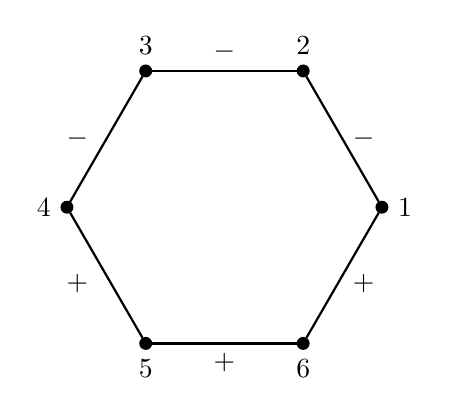
\begin{tikzpicture}
			\tikzstyle{vertex}=[draw, circle, inner sep=0pt, minimum size=.15cm, fill=black]
			\tikzstyle{edge}=[,thick]
			\node[vertex,label=right:1](v1)at(2,0){};
			\node[vertex,label=above:2](v2)at(1,1.73){};
			\node[vertex,label=above:3](v3)at(-1,1.73){};
			\node[vertex,label=left:4](v4)at(-2,0){};
			\node[vertex,label=below:5](v5)at(-1,-1.73){};
			\node[vertex,label=below:6](v6)at(1,-1.73){};
			%\node[vertex,label=center:7](v7)at(-2,1){};
			%\node[vertex,label=center:8](v8)at(-1,2){};
			%\node[vertex,label=center:1](v9)at(12,0){};
			\draw[edge](v1)--node[right, yshift=0cm, xshift=-0cm]{$-$}(v2);
			\draw[edge](v2)--node[above]{$- $}(v3);
			\draw[edge](v3)--node[left, yshift=-0cm, xshift=-0.1cm]{$-$}(v4);
			\draw[edge](v4)--node[left, yshift=-0.1cm, xshift=-0.1cm]{$+$}(v5);
			\draw[edge](v5)--node[below, yshift=-0cm, xshift=0cm]{$+$}(v6);
			\draw[edge](v6)--node[right, yshift=-0.1cm, xshift=0cm]{$+$}(v1);
		\end{tikzpicture} \caption{G}\end{figure}
	Then the path $P_1=\{1,2\}\{2,3\}\{4,3\}$ is a maximal signed negative path and $P_2=\{4,5\}\{5,6\}\{6,1\}$ is a maximal signed positive path.
	
	Suppose $P$ is a matrix property that a real matrix may or may not have. Then a sign pattern $\mathcal{P}$ is said to \textit{require} $P$ if every real matrix in $\mathcal{Q}(\mathcal{P})$ satisfies the property $P$, or to \textit{allow} $P$ if some real matrix in $\mathcal{Q}(\mathcal{P})$ satisfies $P$.
	
	
	
	Let $A$ be an $n\times n$ real matrix, the \textit{inertia} of $A$,  denoted by $\In(A)$, is the triple of nonnegative numbers $\In(A)=(i_+(A), i_-(A),i_0(A))$, where $i_+(A)$, $i_-(A)$ and $i_0(A)$ denote the number of eigenvalues of $A$ with positive, negative and zero real parts, respectively. Furthermore, $\RIn(A) = (i_+(A), i_-(A), i_z(A), 2i_{p}(A))$ is the \textit{refined inertia} of $A$, where $i_z(A)$, $2i_{p}(A)$ represent the number of zero eigenvalues, nonzero purely imaginary eigenvalues of A, respectively. The \textit{eigenvalue frequency} of an $n\times n$ real matrix $A$ is defined as the ordered pair $S_A=(k,n-k)$, where $k$ is the number of real eigenvalues of $A$ and $n-k$ is the number of nonreal eigenvalues of $A$. 
	
	
	
	For a sign pattern $\mathcal{P} \in \mathcal{Q}_n$, the inertia of $\mathcal{P}$ is defined as $\In(\mathcal{P})=\{\In(A): A\in \mathcal{Q}(\mathcal{P})\}$ and the refined
	inertia of $\mathcal{P}$ is defined as $\RIn(\mathcal{P})=\{\RIn(A): A\in \mathcal{Q}(\mathcal{P})\}$. The sign pattern $\mathcal{P}$ is called $k$-consistent, for some fixed nonnegative integer $k$ with $0\leq k \leq n$, if $S_A=(k,n-k)$ for all $A\in \mathcal{Q}(\mathcal{P})$. If $\mathcal{P}$ is $k$-consistent, then we write $S_{\mathcal{P}}=(k,n-k)$. Additionally, $\mathcal{P}$ is said to be consistent if it is $k$-consistent for some integer $k$, where $0\leq k\leq n$.
	
	Let $A$ be a square matrix of order $n$. If $\alpha$, $\beta$ are subsets of $\{1,2,...,n\}$, then $A[\alpha,\beta]$ denotes the submatrix of $A$ with rows, columns corresponding to the indices in $\alpha, \beta$, respectively. In particular, $A[\alpha]$ denotes $A[\alpha, \alpha]$.
	
	
	%In \cite{1988} Eschenbach et al. proposed the problem of characterizing $k$-consistent sign patterns for $0<k<n$. In \cite{1991}, the authors characterized all $n\times n$ consistent sign patterns $\mathcal{P}$ for which $S_{\mathcal{P}}=(0,n)$ or $(n,0)$. For sign pattern matrices of odd order, the following results are by Eschenbach \cite{1993a}.
	
	If $\mathcal{P}_1$, $\mathcal{P}_2$ are two sign patterns, then the patterns are said to be equivalent if one can be obtained from
	the other through a series of permutation similarity, signature similarity, negation, and transposition. Being
	equivalent, $\mathcal{P}_1$ requires a unique inertia if and only if $\mathcal{P}_2$ requires a unique inertia.
	
	Let $\mathcal{P}_1, \mathcal{P}_2 \in \mathcal{Q}_n$ be two sign patterns. We say that $\mathcal{P}_2$ is a \textit{superpattern} of $\mathcal{P}_1$ if $\mathcal{P}_2$ can be obtained from $\mathcal{P}_1$ by replacing some (possibly none) of the zero entries of $\mathcal{P}_1$ with either $+$ or $-$. In this case, $\mathcal{P}_1$ is called a \textit{subpattern} of $\mathcal{P}_2$.
	
	
	
	Suppose $\mathcal{P}=(p_{ij})\in \mathcal{Q}_n$ is an irreducible sign pattern whose underlying signed directed graph $D$ contains a simple $k$-cycle $\gamma$.  Define the real matrix $B_\gamma(0)=(b_\gamma(0)_{ij})$ by
	\begin{equation} \label{e1}
		b_{\gamma}(0)_{ij}= \begin{cases}
			1 & \text{if}\ p_{ij}=+ ~\text{and}~ \text{is}~ \text{in}~ \gamma \\
			-1 & \text{if}\ p_{ij}=- ~\text{and}~ \text{is}~ \text{in}~ \gamma \\
			0 & \text{elsewhere,}
		\end{cases}
	\end{equation}
	and define the perturbed matrix $B_\gamma(\epsilon)=(b_\gamma(\epsilon)_{ij})$ by
	\begin{equation} \label{e2}
		b_{\gamma}(\epsilon)_{ij}= \begin{cases}
			b_\gamma(0)_{ij} & \text{if}\ p_{ij}~ \text{is}~ \text{in}~ \gamma \\
			\epsilon & \text{if}\ p_{ij}=+ ~\text{and}~ \text{is}~\text{not}~ \text{in}~ \gamma \\
			-\epsilon & \text{if}\ p_{ij}=- ~\text{and}~ \text{is}~ \text{not}~\text{in}~ \gamma \\
			0 & \text{elsewhere,}
		\end{cases}
	\end{equation}
	for some $\epsilon>0$. Since $B_\gamma(0)$ has $k$ nonzero algebraically simple eigenvalues which are the $k$-th complex roots of $+1$, $-1$ depending on $\sgn(\gamma)$, and the eigenvalues of a real matrix are continuous functions of the entries of the matrix, for $\epsilon>0$ sufficiently small, the perturbed matrix $B_\gamma(\epsilon)\in \mathcal{Q}(\mathcal{P})$ has $k$ algebraically simple nonzero eigenvalues close to the nonzero eigenvalues of $B_\gamma(0)$. If $\gamma$ is a negative even $k$-cycle, then $B_\gamma(0)$ has $k$ nonreal algebraically simple eigenvalues, thus, for $\epsilon>0$, sufficiently small the matrix $B_\gamma(\epsilon)$ has $k$ distinct nonreal eigenvalues. Similarly, if $\gamma$ is a positive even $k$-cycle then $B_\gamma(0)$ has algebraically simple real eigenvalues $1$ and $-1$, so for $\epsilon>0$, sufficiently small $B_\gamma(\epsilon)$ has two algebraically simple real eigenvalues close to $1$ and $-1$.
	Similarly if $\Gamma$ is a composite cycle in $D$, we can define $B_\Gamma(0)$ and $B_{\Gamma}(\epsilon)$ satisfying similar properties. 
	
	
	%In \cite{2022}, Breen et al. characterized all $2\times 2$ and $3\times 3$ irreducible sign patterns $\mathcal{P}$ according to the value of $q(\mathcal{P})$. In \cite{2002}, the authors proved some necessary and sufficient conditions for an $n\times n$ sign pattern $\mathcal{P}$ for which $q(\mathcal{P})=n$.
	
	Assume $\mathcal{P}\in \mathcal{Q}_n$ is a sign pattern such that the maximal cycle length in the signed directed graph of $\mathcal{P}$ is $m$. Let $B\in \mathcal{Q}(\mathcal{P})$ then the characteristic polynomial of $B$ (denoted by $\Ch_B(x)$) is given by $$\Ch_B(x)=x^n-E_1(B)x^{n-1}+E_2(B)x^{n-2}-\cdots+(-1)^mE_m(B)x^{n-m},$$ where $E_k(B)$ for $1\leq k\leq m$, is the sum of all cycles (simple or composite) of length $k$ in $B$ properly signed.
	Let $V_+(x)$ be the variation of signs in the terms of $\Ch_B(x)$ for $x>0$, and let $V_-(x)$ be the variation of signs in the terms of $\Ch_B(x)$ for $x<0$. Then, by Descartes' rule of signs, the number of positive (negative) roots of $\Ch_B(x)$ is either equal to $V_+(x)$ ($V_-(x)$, respectively) or is less than it by an even number. For example, consider $\Ch_B(x)=a_3x^3+a_2x^2+a_1x+a_0$, for some real matrix $B$ and $a_i\in \mathbb{R}$, $i=0,1,2,3$. Then, 
	$$
	\sgn(\Ch_B(x)) = \begin{cases} 
		(\sgn(a_3))(+)+(\sgn(a_2))(+)+(\sgn(a_1))(+)+(\sgn(a_0)) & \text{if} ~ x> 0 \\
		(\sgn(a_3))(-)+(\sgn(a_2))(+)+(\sgn(a_1))(-)+(\sgn(a_0)) & \text{if} ~x<0,
	\end{cases}
	$$ where the notation $(\sgn(a_i))(\cdot)$ in the $i$-th position represents the product of $\sgn(a_i)$ and the sign of $x^i$ for $3\geq i\geq 0$, depending on whether $x>0$ or $x<0$.
	If \( V_+(x) = 1 \) and \( V_-(x) = 2 \) for some \( a_i \in \mathbb{R} \), \( i = 0, 1, 2, 3 \), then the number of positive roots of $\Ch_B(x)$ is exactly one, and the number of negative roots is either two or zero.
	
	
	Symmetric sign patterns requiring a unique inertia has been studied in \cite{2001, 2001a, 2018, 2024}. For instance, in \cite{2001}, the authors characterized symmetric sign patterns that require a unique inertia in terms of the symmetric minimal rank and symmetric maximal rank. Also, sufficient conditions for symmetric tree sign patterns to require a unique inertia based on the sign and position of the loops in the underlying graph were given in \cite{2018, 2024}. In \cite{2001a}, Hall and Li characterized all irreducible symmetric tridiagonal sign patterns requiring a unique inertia. Lin et al. \cite{2018} characterized all irreducible sign patterns of order 2 and 3 that require a unique inertia.
	
	
	
	
	
	In Section \ref{s2}, to begin with, we consider irreducible combinatorially symmetric tree sign patterns with a $0$-diagonal and obtain some necessary conditions for such patterns to require a unique inertia based on the multiplicity of eigenvalues with zero real part. Next, we shift our focus to a particular type of tree sign pattern, the tridiagonal sign patterns with a $0$-diagonal, and we obtain necessary conditions based on the number of maximal signed paths of odd length that are allowed by the sign pattern for requiring a unique inertia. We also identify certain patterns which cannot occur as subpatterns of tridiagonal sign patterns requiring a unique inertia. 
	In Section \ref{s4}, we investigate irreducible combinatorially symmetric sign patterns whose underlying graphs contain cycles but no loops. We derive necessary conditions for such sign patterns to require a unique inertia based on the number of negative edges and other combinatorial properties of the cycles in the underlying graphs.
	
	We conclude this paper with interesting results which follow from those obtained in this paper, but could not be included in this manuscript. In Section \href{https://arxiv.org/abs/2508.21509v1}{4}, we also include problems which come as natural extensions of the results obtained in this paper and that pave the way for future research in this topic. 
	
	
	
	\section{Tree and path sign patterns with a $0$-diagonal requiring a unique inertia} \label{s2}
	
	As mentioned earlier, all the patterns in this paper are assumed to be combinatorially symmetric.
	In this section, to begin with, we show that if a tree sign pattern with a $0$-diagonal has no repeated eigenvalues with zero real part, then it has a unique inertia. 
	We also establish that for tridiagonal sign patterns with a $0$-diagonal, if there are no repeated zero eigenvalues, then it requires a unique inertia.
	The relationship between tridiagonal patterns requiring a unique inertia with the consistency of certain associated patterns were useful in identifying certain combinatorial structures of such patterns requiring a unique inertia.
	
	
	
	
	
	\begin{lemma} \label{lem1}
		Suppose that $f(x)$ is a real polynomial of even degree $n$, consisting only of even powers of $x$. If $\lambda$ is a root of $f(x)$ with multiplicity $m$, then $-\lambda$ is also a root of $f(x)$ with multiplicity $m$.
	\end{lemma}
	\begin{proof}
		Since $\lambda$ is a root of $f(x)$ with multiplicity $m$, so $f(x)=(x-\lambda)^mg(x)$ where $g(x)$ is a polynomial of degree $n-m$ with $g(\lambda)\neq 0$. Since $f(x)$ consists only of even powers of $x$, $$f(x)=f(-x)=(-1)^m(x+\lambda)^mg(-x).$$
		Thus $(x+\lambda)^m$ is also a factor of $f(x)$, so $f(x)=(x-\lambda)^m(x+\lambda)^mg^{(1)}(x)$. Therefore, $-\lambda$ is a root of $f(x)$ with multiplicity at least $m$. If $-\lambda$ is a root of $f(x)$ with multiplicity greater than $m$, then similarly $\lambda$ is also a root of $f(x)$ with multiplicity greater than $m$, which is a contradiction. Therefore, if $\lambda$ is a root of $f(x)$ with multiplicity $m$, then $-\lambda$ is also a root of $f(x)$ with multiplicity $m$.
	\end{proof}
	
	\begin{cor} \label{xlem1}
		Suppose that $f(x)$ is a real polynomial of odd degree $n$, consisting only of odd powers of $x$. If $\lambda$ is a root of $f(x)$ with multiplicity $m$, then $-\lambda$ is also a root of $f(x)$ with multiplicity $m$.
	\end{cor}
	\begin{proof}
		Since $f(x)$ is a real polynomial of odd degree $n$, consisting only of odd powers of $x$, we have $f(x)=xg(x)$, where $g(x)$ is a real polynomial of even degree that consists only of even powers of $x$. Hence, by Lemma~\ref{lem1}, the result follows.
	\end{proof}
	
	
	Since for a tree sign pattern $\mathcal{P} \in \mathcal{Q}_n$ with a $0$-diagonal, the characteristic polynomial $\Ch_B(x)$ of $B \in \mathcal{Q}(\mathcal{P})$ consists only of even powers of $x$ when $n$ is even and only odd powers of $x$ when $n$ is odd, Lemma \ref{lem1} and its corollary give the following result.
	\begin{cor}\label{c1}
		Suppose that $\mathcal{P}\in \mathcal{Q}_n$ is a tree sign pattern with a $0$-diagonal and $B\in \mathcal{Q}(\mathcal{P})$. If $\lambda$ is an eigenvalue of $B$ with algebraic multiplicity $m$, then $-\lambda$ is also an eigenvalue of $B$ with algebraic multiplicity $m$.
	\end{cor}
	%	Let \textbf{$n_r(\mathcal{P})$} (respectively, $n_c(\mathcal{P})$) be the maximum number of real (respectively, non-real) eigenvalues allowed by $\mathcal{P}\in \mathcal{Q}_n$. Eschenbach et al. \cite{1}, proved that \textcolor{red}{(page-465)} $\mathcal{P}$ is consistent if and only if $n_r(\mathcal{P})+n_c(\mathcal{P})=n$.
	The following result is by Eschenbach et al. \cite{1}.
	\begin{lemma}[Lemma 1.5, \cite{1}] \label{l1}
		If an $n\times n$ sign pattern matrix $\mathcal{A}$ does not allow repeated real eigenvalues, then $\mathcal{A}$ is consistent.
	\end{lemma}
	
	
	The following is a similar sufficient condition for tree sign patterns with a $0$-diagonal to require a unique inertia.
	
	\begin{theorem} \label{l3.3ne}
		If $\mathcal{P}\in \mathcal{Q}_n$ is a tree sign pattern with a $0$-diagonal such that it does not allow repeated eigenvalues with zero real part, then $\mathcal{P}$ requires a unique inertia.
	\end{theorem}
	\begin{proof}
		Let $B_1,B_2\in \mathcal{Q}(\mathcal{P})$ be arbitrary. Define $$B(t)=(1-t)B_1+tB_2$$ and $\In(B(t))=(i_+(t),i_-(t),i_0(t))$, where $i_+(t)+i_-(t)+i_0(t)=n$. If $b_1=b_2$, then $(1-t)b_1+tb_2=b_1$ for all $t$. Also, if $b_1 \neq b_2$ and $\sgn(b_1)=\sgn(b_2)$, then $b_1+t(b_2-b_1)$ has the same sign as $b_1$ for all $t\in [0-\delta, 1+\delta]$, where $$0<\delta<\frac{1}{|b_2-b_1|}\min\{|b_1|,|b_2|\}.$$ Therefore, for sufficiently small $\delta>0$, $B(t)\in \mathcal{Q}(\mathcal{P})$ for all $t\in [0-\delta,1+\delta]$. Let $c\in [0,1]$ and $B(c)$ have $i_0(c)$ eigenvalues with zero real part, then by hypothesis, they are all distinct. Suppose that $\lambda_1, \lambda_2,...,\lambda_{i_0(c)}$ are the eigenvalues with zero real part and let the other eigenvalues of $B(c)$ be $\lambda_{i_0(c)+1}, \lambda_{i_0(c)+2},...,\lambda_n$. Consider 
		\begin{align*}
			\epsilon_1&=\min\left\{ \frac{|\lambda_i-\lambda_j|}{2}: 1\leq i<j\leq n~ \text{and} ~ \lambda_i\neq \lambda_j\right\},\\ \epsilon_2&=\min\{|Re(\lambda_j)|: i_0(c)+1\leq j\leq n\},\\ \epsilon_c&=\min\{\epsilon_1,\epsilon_2\}~ \text{and} ~ D_i=\{c\in \mathbb{C}: |x-\lambda_i|<\epsilon_c\}.
		\end{align*}
		Then we have $D_i\cap D_j=\emptyset$ whenever $\lambda_i\neq \lambda_j$. Since the eigenvalues of $B(t)$ are continuous functions of $t$, therefore there exists a $\delta_c>0$ such that for all $i$, $1\leq i\leq i_0(c)$, the disk $D_i$ contains exactly one eigenvalue of $B(t)$ and for each $j$, $i_0(c)+1\leq j\leq n$, if $m_j$ is the algebraic multiplicity of $\lambda_j$, then the disk $D_j$ contains exactly $m_j$ eigenvalues of $B(t)$ whenever $|t-c|<\delta_c$. Since $B(t)$ is a real matrix whose underlying signed undirected graph is a tree with no loop, by Corollary \ref{c1} if $\lambda$ is an eigenvalue of $B(t)$, then $-\lambda$ is also an eigenvalue of $B(t)$, so the eigenvalue of $B(t)$ in $D_i$, $1\leq i\leq i_0(c)$ has zero real part.
		%*imp*- that the coefficients of the characteristic polynomial are real. so, non-real eigenvalues occur in complex conjugate pairs.
		Also, for $i_0(c)+1\leq i\leq n$, since $D_i$ does not intersect the imaginary axis, we conclude that the real part of each eigenvalue of $B(t)$ in $D_i$ has the same sign as $Re(\lambda_i)$. Thus, $\In(B(t))=\In(B(c))$, for all $t\in(c-\delta_c,c+\delta_c)$. Since $c\in [0,1]$ is arbitrary, $\{(c-\delta_c,c+\delta_c)\}_c$ forms an open cover of $[0,1]$, which has a finite subcover. Let $\{(c-\delta_c,c+\delta_c)\}_{c\in S}$ where $S=\{c_1,c_2,...,c_l\}$ be a finite subcover of $[0,1]$. Since $\In(B(t))$ is constant in each $(c-\delta_c,c+\delta_c)$, $c\in S$, $\In(B(t))$ is constant for all $t\in [0,1]$. Therefore, $\In(B_1)=\In(B_2)$ and $\mathcal{P}$ require a unique inertia.
	\end{proof}
	The above result is not true in general if the underlying signed undirected graph of the tree sign pattern $\mathcal{P}$ contains loops.
	\begin{eg}
		Let $$\mathcal{P}=\begin{bmatrix}
			+&+\\+&+
		\end{bmatrix}.$$ Then $\text{trace}(A)>0$ for all $A\in \mathcal{Q}(\mathcal{P})$, therefore $\mathcal{P}$ does not allow repeated eigenvalues with zero real part. However, $\mathcal{P}$ does not require a unique inertia, since $(2,0,0),(1,0,1)\in \In(\mathcal{P})$.   
	\end{eg}
	Also, the conclusion of Theorem \ref{l3.3ne} is not true if $\mathcal{P}$ is not a tree sign pattern, even if it has a $0$-diagonal.
	\begin{eg}\label{example2.6}
		Let $$\mathcal{P}=\begin{bmatrix}
			0&+&-\\-&0&+\\+&-&0
		\end{bmatrix}.$$ Suppose that $$B=\begin{bmatrix}
			0&a_1&-a_2\\-a_3&0&a_4\\a_5&-a_6&0
		\end{bmatrix}\in \mathcal{Q}(\mathcal{P}),$$
		where $a_i>0$ for $i=1,2,...,6$. Then $\Ch_B(x)=x^3+(a_1a_3+a_2a_5+a_4a_6)x+(a_2a_3a_6-a_1a_4a_5)$. Then we have the following cases.
		\begin{itemize}
			\item[i.] If $a_2a_3a_6-a_1a_4a_5>0$, then
			$$
			\sgn(\Ch_B(x)) = \begin{cases} 
				(+)+(+)(+)+(+) & \text{if} ~ x> 0 \\
				(-)+(+)(-)+(+) & \text{if} ~x<0.
			\end{cases}
			$$
			So $V_+(x)=0$ and $V_-(x)=1$, and by Descartes' rule of signs, $\Ch_B(x)$ has exactly one negative root and no positive or zero root.
			\item[ii.] If $a_2a_3a_6-a_1a_4a_5<0$, then
			$$
			\sgn(\Ch_B(x)) = \begin{cases} 
				(+)+(+)(+)+(-) & \text{if} ~ x> 0 \\
				(-)+(+)(-)+(-) & \text{if} ~x<0.
			\end{cases}
			$$
			So $V_+(x)=1$ and $V_-(x)=0$, and by Descartes' rule of signs, $\Ch_B(x)$ has exactly one positive root and no negative or zero root.
			\item[iii.] If $a_2a_3a_6-a_1a_4a_5=0$, then
			$\Ch_B(x)=x(x^2+(a_1a_3+a_2a_5+a_4a_6))$, thus $0$ is the only real root of $\Ch_B(x)$.
		\end{itemize} Hence, any $B\in \mathcal{Q}(\mathcal{P})$ has exactly one real eigenvalue. Therefore, $\mathcal{P}$ has all distinct eigenvalues and does not allow repeated eigenvalues with zero real part. However,
		\begin{itemize}
			\item[i.] if $a_i=1$ for all $i=1,2,...,6$, then $\In(B)=(0,0,3),$
			\item[ii.] if $a_1=2$ and $a_i=1$ for $i=2,3,...,6$, then $\In(B)=(1,2,0).$
		\end{itemize}
		So, $\mathcal{P}$ does not require a unique inertia. 
	\end{eg}
	
	
	
	
	
	The converse of Theorem \ref{l3.3ne} is not true for tree sign patterns with a $0$-diagonal, as the following example shows.
	\begin{eg}
		Let $$\mathcal{P}=\begin{bmatrix}
			0&+&+&+\\+&0&0&0\\+&0&0&0\\+&0&0&0
		\end{bmatrix}.$$ Then $\mathcal{P}$ is a sign symmetric tree sign pattern with zero diagonal, and by Remark~4.1\cite{2018}, every matrix $B\in\mathcal{Q}(\mathcal{P})$ is similar to a symmetric matrix, so by Theorem 4.3\cite{2001}, $\mathcal{P}$ requires a unique inertia. However, for $B\in \mathcal{Q(\mathcal{P})}$ with all nonzero entries equal to $1$, the eigenvalues of $B$ are $0,0,\sqrt{3},-\sqrt{3}$. Here, the eigenvalue $0$ is repeated.
	\end{eg}
	%*****delete******However, the converse of Lemma \ref{l3.3ne} is true for all tridiagonal sign patterns of order at most $5$, as proved in Corollary \ref{cor3.8n}.
	
	
	%\textbf{ The next theorem gives a necessary condition for irreducible tridiagonal sign patterns with a $0$-diagonal to require a unique inertia. First, we need to prove a lemma.}
	
	
	For symmetric sign patterns whose underlying graphs are trees, Hall et al. \cite{2001} obtained the following result.
	\begin{theorem}[Theorem 4.5, \cite{2001}]  Let $\mathcal{A}$ be a symmetric tree sign pattern, with the maximum length of the cycles in A equal to $m\geq 1$. Then $\mathcal{A}$ requires a unique inertia if and only if all the terms in $E_m(B)$ have the same sign for any $B \in \mathcal{Q}(\mathcal{A})$. In this case, $\mathcal{A}$ requires rank $m$.
	\end{theorem}
	
	
	We investigate the above result for general sign patterns which are not necessarily symmetric.
	
	\begin{lemma}\label{xnl1}
		Let $\mathcal{P}\in \mathcal{Q}_n$ be a sign pattern, whose underlying signed directed graph is $D$. Suppose that the maximum length of a composite cycle in $D$ is $m$, $m\geq 2$, then $\mathcal{P}$ requires a unique inertia only if all the composite cycles in $D$ of length $m$ have the same sign.
	\end{lemma}
	\begin{proof}
		Since the maximum length of a composite cycle in $D$ is $m$, the characteristic polynomial of any $B\in \mathcal{Q}(\mathcal{P})$ is given by, 
		$$\Ch_B(x)=x^n-E_1(B)x^{n-1}+E_2(B)x^{n-2}-\cdots+(-1)^mE_m(B)x^{n-m},$$
		where $E_k(B)$ for $1\leq k\leq m$ is the sum of all cycles (simple or composite) of length $k$ in $B$ properly signed. Suppose $\Gamma_1$, $\Gamma_2$ are two oppositely signed composite cycles in $D$ of length $m$. Then, by emphasizing the entries of $\mathcal{P}$ corresponding to $\Gamma_1$, $\Gamma_2$, we construct matrices $B_{\Gamma_1}(\epsilon), B_{\Gamma_2}(\epsilon') \in \mathcal{Q}(\mathcal{P})$ as in \ref{e2}, for some $\epsilon, \epsilon'>0$, such that $E_m(B_{\Gamma_1}(\epsilon))=-E_m(B_{\Gamma_2}(\epsilon'))$.
		
		Since $E_m(B)$ is equal to the product of all the nonzero eigenvalues of $B$, for any $B\in \mathcal{Q}(\mathcal{P})$ and the nonreal eigenvalues of $B$ occur in conjugate pairs, $E_m(B_{\Gamma_1}(\epsilon))=-E_m(B_{\Gamma_2}(\epsilon'))$ implies that $i_-(B_{\Gamma_1}(\epsilon))\neq i_-(B_{\Gamma_2}(\epsilon'))$. Therefore, $\mathcal{P}$ does not require a unique inertia.
	\end{proof}
	
	The converse of Theorem \ref{xnl1} is not true in general, as the following example shows.
	\begin{eg}\label{xxeg2.2}
		Suppose that $\mathcal{P}$ is an irreducible combinatorially symmetric sign pattern with a $0$-diagonal, whose underlying signed directed graph $D$ is given in Fig.\ref{fignx1}.
		\begin{figure}[H]
			\centering
			\begin{minipage}{.45\textwidth}
				\vspace{-1cm}
				\[
				\mathcal{P}=\begin{bmatrix}
					0 & + & 0 & + \\
					- & 0 & + & 0 \\
					0 & + & 0 & - \\
					+ & 0 & + & 0
				\end{bmatrix}
				\]
			\end{minipage}
			\hspace{0.05\textwidth}
			\begin{minipage}{.45\textwidth}
				\centering
				\tikzset{node distance=1cm}
				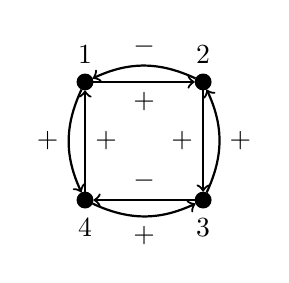
\begin{tikzpicture}[
					vertex/.style={draw, circle, inner sep=0pt, minimum size=2mm, fill=black},
					edge/.style={thick, ->}
					]
					% Vertices
					\node[vertex,label=above:1] (v1) at (-0.75, 0.75) {};
					\node[vertex,label=above:2] (v2) at ( 0.75, 0.75) {};
					\node[vertex,label=below:3] (v3) at ( 0.75,-0.75) {};
					\node[vertex,label=below:4] (v4) at (-0.75,-0.75) {};
					
					% Edges
					\draw[edge] (v1) -- node[below] {$+$} (v2);
					\draw[edge, bend right=25] (v2) to node[above] {$-$} (v1);
					
					\draw[edge] (v2) -- node[left] {$+$} (v3);
					\draw[edge, bend right=25] (v3) to node[right] {$+$} (v2);
					
					\draw[edge] (v3) -- node[above] {$-$} (v4);
					\draw[edge, bend right=25] (v4) to node[below] {$+$} (v3);
					
					\draw[edge] (v4) -- node[right] {$+$} (v1);
					\draw[edge, bend right=25] (v1) to node[left] {$+$} (v4);
				\end{tikzpicture}
				\caption{Signed directed graph \(D\) of \(\mathcal{P}\).}
				\label{fignx1}
			\end{minipage}
			
		\end{figure}
		
		Then the maximum length of a composite cycle in $D$ is $4$, and all such cycles have the same sign, which is positive. However, consider	$$\begin{bmatrix}
			0&a&0&b\\ -c&0&d&0\\ 0&e&0&-f\\ g&0&h&0
		\end{bmatrix}\in \mathcal{Q}(\mathcal{P}), ~\text{where}~ a,b,c,d,e,f,g,h>0.$$ \begin{itemize}
			\item[i.] Let $B_1 \in \mathcal{Q}(\mathcal{P})$ with $a = b = c = d = e = f = g = h = 1$. Then $\sigma(B_1) = \{1+i, 1-i,-1-i,-1+i\}$, and $\In(B_1) = (2, 2, 0)$.
			\item[ii.] Let $B_2 \in \mathcal{Q}(\mathcal{P})$ with $a = 11$, $ b = c = d = e = f = g = h = 1$. Then $\sigma(B_2) = \{2i,-2i,\sqrt{6}i,-\sqrt{6}i\}$, and $\In(B_2) = (0, 0, 4)$.
		\end{itemize}
		Therefore, $\mathcal{P}$ does not require a unique inertia.
	\end{eg}
	
	\begin{theorem} \label{l3.1n}
		If $\mathcal{P}\in \mathcal{Q}_n$ is an irreducible tridiagonal sign pattern with a $0$-diagonal such that $\mathcal{P}$ allows repeated zero eigenvalues, then $\mathcal{P}$ does not require a unique inertia.
	\end{theorem}
	\begin{proof} Since $\mathcal{P}$ allows zero eigenvalues, $n$ must be odd. Therefore, the maximum length of a composite cycle in the signed directed graph $D$ of $\mathcal{P}$ is $n-1$, which is even. Since $\mathcal{P}$ allows repeated zero eigenvalues, the underlying signed directed graph $D$ of $\mathcal{P}$ contains at least two composite cycles of length $n - 1$ with opposite signs.
		Therefore, from Lemma~\ref{xnl1}, it follows that $\mathcal{P}$ does not require a unique inertia.
		%Let $\Gamma_1=\alpha_1\alpha_2\cdots \alpha_{\frac{n-1}{2}}$ and $\Gamma_2=\beta_1\beta_2\cdots \beta_{\frac{n-1}{2}}$ be two composite cycles in $D$ of length $n-1$, oppositely signed, where each $\alpha_i$, $\beta_j$ is a $2$-cycle in $D$.
		%Since the maximum length of a composite cycle in $D$ is $n - 1$, and $\Gamma_1$, $\Gamma_2$ are two of such oppositely signed cycles, it 
	\end{proof}
	
	The converse of Theorem~\ref{l3.1n} is not true in general, as the following example shows.
	\begin{eg} Let $$\mathcal{P}=\begin{bmatrix}
			0&-&0&0\\ +&0&+&0\\ 0&+&0&-\\ 0&0&+&0
		\end{bmatrix}$$ be an irreducible tridiagonal sign pattern with a $0$-diagonal. Any real matrix $B\in \mathcal{Q}(\mathcal{P})$ is similar to	$$\begin{bmatrix}
			0&-1&0&0\\ a&0&1&0\\ 0&b&0&-1\\ 0&0&c&0
		\end{bmatrix}~\text{where} ~a,b,c>0.$$ Since $\det(B)\neq 0$, $\mathcal{P}$ does not allow any zero eigenvalue. However,
		\begin{itemize}
			\item[i.] let $B_1 \in \mathcal{Q}(\mathcal{P})$ with $a=c=1$, $b=4$. Then $\sigma(B_1)=\{1, 1, -1,-1\}$, and hence $In(B_1)=(2,2,0)$,
			\item[ii.] let $B_2 \in \mathcal{Q}(\mathcal{P})$ with $a=8$, $b=c=2$. Then $\sigma(B_2)=\{2i,2i, -2i,  -2i\}$, and hence $\In(B_2) = (0, 0, 4)$.
		\end{itemize} Hence, $\mathcal{P}$ does not requires a unique inertia.
	\end{eg}
	
	
	
	The conclusion of Theorem \ref{l3.1n} is not necessarily true for tree sign patterns of odd order with a $0$-diagonal.
	\begin{eg}
		Let $$\mathcal{P}=\begin{bmatrix}
			0&+&+&+&+\\+&0&0&0&0\\+&0&0&0&0\\+&0&0&0&0\\+&0&0&0&0
		\end{bmatrix}.$$ Then $rank(B)=2$ for all $B\in \mathcal{Q}(\mathcal{P})$, so $\mathcal{P}$ allows repeated zero eigenvalues. However, $\mathcal{P}$ is a symmetric tree sign pattern with a $0$-diagonal, and by Remark~4.1\cite{2018}, every matrix $B\in\mathcal{Q}(\mathcal{P})$ is similar to a symmetric matrix, so by Theorem 4.3\cite{2001}, $\mathcal{P}$ requires a unique inertia.
	\end{eg}
	
	
	
	
	%To state the next results, we need the following definition.
	\begin{definition}
		Let $\mathcal{P}\in \mathcal{Q}_n$ be a tree sign pattern with a $0$-diagonal, with the underlying signed undirected graph $G$. Then $\mathcal{P}_-$ is defined to be the sign pattern whose underlying signed undirected graph $G_-$ is obtained from $G$ by taking the opposite sign of each signed edge of $G$.
	\end{definition}
	
	\begin{eg} Let $\mathcal{P}\in \mathcal{Q}_n$ be a tree sign pattern with a $0$-diagonal, whose underlying signed undirected graph is $G$  given in Fig.\ref{figx1}.
		\begin{figure}[H]
			\centering
			\begin{minipage}{.45\textwidth}
				\vspace{-1cm}
				\[
				\mathcal{P}=\begin{bmatrix}
					0 & + & 0 & 0 \\
					+ & 0 & + & + \\
					0 & - & 0 & 0 \\
					0 & + & 0 & 0
				\end{bmatrix}
				\]
			\end{minipage}
			\hspace{0.05\textwidth}
			\begin{minipage}{.45\textwidth}
				\centering
				\tikzset{node distance=1cm}
				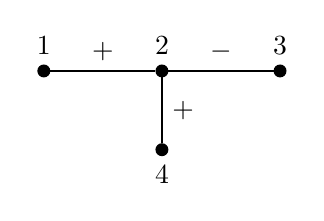
\begin{tikzpicture}[
					vertex/.style={draw, circle, inner sep=0pt, minimum size=.15cm, fill=black},
					edge/.style={thick}
					]
					% Vertices
					\node[vertex,label=above:1] (v1) at (-1.5,0) {};
					\node[vertex,label=above:2] (v2) at (0,0) {};
					\node[vertex,label=above:3] (v3) at (1.5,0) {};
					\node[vertex,label=below:4] (v4) at (0,-1) {};
					
					% Edges
					\draw[edge] (v1) -- node[above] {$+$} (v2);
					\draw[edge] (v2) -- node[above] {$-$} (v3);
					\draw[edge] (v4) -- node[right] {$+$} (v2);
				\end{tikzpicture}
				\caption{Signed undirected graph $ G$ of $\mathcal{P}$.}
				\label{figx1}
			\end{minipage}
		\end{figure}
		
		
		
		Then the underlying graph corresponding to $\mathcal{P}_-$ is $G_-$ given in Fig.\ref{fign2}.
		\begin{figure}[H]
			\centering
			% Left minipage: matrix
			\begin{minipage}{0.45\textwidth}
				\vspace{-1cm}
				\[
				\mathcal{P}_-=
				\begin{bmatrix}
					0 & + & 0 & 0 \\
					- & 0 & + & + \\
					0 & + & 0 & 0 \\
					0 & - & 0 & 0
				\end{bmatrix}
				\]
			\end{minipage}\hfill
			% Right minipage: TikZ figure
			\begin{minipage}{0.45\textwidth}
				\centering
				\tikzset{
					vertex/.style={draw, circle, inner sep=0pt, minimum size=.15cm, fill=black},
					edge/.style={thick}
				}
				\begin{tikzpicture}
					\node[vertex,label=above:1](v1)at(-1.5,0){};
					\node[vertex,label=above:2](v2)at(0,0){};
					\node[vertex,label=above:3](v3)at(1.5,0){};
					\node[vertex,label=below:4](v4)at(0,-1){};
					
					\draw[edge](v1)--node[above]{$-$}(v2);
					\draw[edge](v2)--node[above]{$+$}(v3);
					\draw[edge](v4)--node[right]{$-$}(v2);
				\end{tikzpicture}
				\caption{Signed undirected graph $G_-$ of $\mathcal{P}_-$.}
				\label{fign2}
			\end{minipage}
		\end{figure}
		
	\end{eg}
	\begin{lemma} \label{3.1} Let $\mathcal{P}\in \mathcal{Q}_n$ be a tree sign pattern with a $0$-diagonal.
		If $\lambda$ is an eigenvalue of $B=[b_{ij}]\in \mathcal{Q}(\mathcal{P})$ with algebraic multiplicity $m$, then $i\lambda$ is an eigenvalue of $B_-=[b^-_{ij}] \in \mathcal{Q}(\mathcal{P}_-)$ with algebraic multiplicity $m$, where $|b_{ij}|=|b^-_{ij}|$ for all $i,j$.
	\end{lemma}
	\begin{proof}
		Suppose that $t$ is the maximum length of a composite cycle in the underlying signed directed graph $D$ of $\mathcal{P}$. Then the characteristic polynomial of $B$ is $$\Ch_B(x)=x^n-E_1(B)x^{n-1}+E_2(B)x^{n-2}-\cdots+(-1)^tE_t(B)x^{n-t},$$ where $E_k(B)$ for $1\leq k\leq t$, is the sum of all the cycles (simple or composite) of length $k$ in $B$, properly signed. 
		
		Let $n$ be even. Since $\mathcal{P}$ is a tree sign pattern of even order, $E_k(B)=0$ for all odd $k$. Therefore, $$\Ch_B(x)=x^n+\sum_{k=1}^{\frac{t}{2}}E_{2k}(B)x^{n-2k}.$$
		Since $\mathcal{P}_-$ is obtained from $\mathcal{P}$ by taking the opposite sign of each edge of the underlying signed undirected graph of $\mathcal{P}$, and $|b_{ij}|=|b_{ij}^-|$, we have 
		$$\Ch_{B_-}(x)=x^n+\sum_{k=1}^{\frac{t}{2}}(-1)^kE_{2k}(B)x^{n-2k}.$$
		Therefore, if $\lambda$ is a root of $\Ch_B(x)$ with multiplicity $m$, then $i\lambda$ is a root of $\Ch_{B_-}(x)$ with multiplicity $m$.
		
		If $n$ is odd, then $\Ch_B(x) = x(x^{n-1}+\sum_{k=1}^{\frac{t}{2}}E_{2k}(B)x^{n-2k-1})$. So, the result follows from the previous part.
	\end{proof}
	
	
	
	The following result is by Lin et al. \cite{2018}.
	
	
	\begin{theorem} [Theorem 2.4, \cite{2018}]\label{th4}
		Let $\mathcal{P}$ be an $n \times n$ sign pattern. Then $\mathcal{P}$ requires a unique inertia if and only if $i_0(A)$ is a fixed number for all $A \in \mathcal{Q}(\mathcal{P})$. Moreover, $\mathcal{P}$ requires a unique refined inertia if and only if $i_z(A)$ and $i_p(A)$ are two fixed numbers for all $A \in \mathcal{Q}(\mathcal{P})$.
	\end{theorem}
	
	The following is an immediate consequence of the previous theorem.
	\begin{theorem}\label{lem2}
		Let $\mathcal{P}\in \mathcal{Q}_n$ and $A,B\in \mathcal{Q}(\mathcal{P})$ be such that $i_0(A)+(n-i_0(B))\geq n+1$, then $\mathcal{P}$ does not require a unique inertia. 
	\end{theorem}
	\begin{proof}
		Since $i_0(A)+(n-i_0(B))\geq n+1$, $i_0(A)\neq i_0(B)$, therefore, by Theorem \ref{th4}, $\mathcal{P}$ does not require a unique inertia.
	\end{proof}
	
	%Suppose that $\mathcal{P}$ is an $n\times n$ irreducible tridiagonal sign pattern with $0$-diagonal. We now specify the certain relation between requiring unique inertia and consistency of $\mathcal{P}$ and $\mathcal{P}_-$.
	
	\begin{theorem} \label{th2.3}
		Let $\mathcal{P}\in \mathcal{Q}_n$ be a tree sign pattern with a $0$-diagonal. Then $\mathcal{P}$ requires a unique inertia if and only if $\mathcal{P}_-$ is consistent.
	\end{theorem}
	\begin{proof}
		Suppose that $\mathcal{P}$ requires a unique inertia. By Theorem \ref{th4}, every $A=[a_{ij}]\in \mathcal{Q}(\mathcal{P})$ has a fixed number of eigenvalues with zero real part.  Since $iA$ and $A_-$ have the same characteristic polynomial, $A_-$ has a fixed number of real eigenvalues, where $A_-=[a^-_{ij}]\in \mathcal{Q}(\mathcal{P_-})$ with $|a_{ij}|=|a^-_{ij}|$ for all $i,j$. Since $A\in \mathcal{Q}(\mathcal{P})$ and $A_- \in \mathcal{Q}(\mathcal{P_-})$ are arbitrary, $\mathcal{P}_-$ is consistent.
		
		The converse follows similarly.
	\end{proof}
	%Clearly from the proof of the above theorem it follows.
	
	%	\begin{cor} \label{th5}
		%		Let $\mathcal{P}$ be an $n\times n$ irreducible tridiagonal sign pattern with $0$-diagonal. Then $\mathcal{P}$ requires unique inertia if and only if $\mathcal{P}_-$ is consistent.
		
		%	\end{cor}
	% The following is an immediate consequence of Theorem \ref{th2.3}.
	\begin{cor}\label{c2.2}
		Let $\mathcal{P}\in \mathcal{Q}_n$ be a tree sign pattern with a $0$-diagonal. Then $\mathcal{P}_-$ requires a unique inertia if and only if $\mathcal{P}$ is consistent.
	\end{cor}
	%\begin{proof}
	%    Similar to the proof of Theorem \ref{th2.3}.
	%\end{proof}
	
	
	
	
	
	
	The following result, by Eschenbach et al. \cite{1}, gives a necessary condition for irreducible tridiagonal sign patterns with a $0$-diagonal to be consistent. We give a similar necessary condition for such sign patterns to require a unique inertia.
	
	
	\begin{theorem} [Theorem 2.8, \cite{1}] \label{th11}
		Let $\mathcal{A}$ be an irreducible tridiagonal pattern with a $0$-diagonal. 
		Then $\mathcal{A}$ is consistent only if the signed undirected graph of $\mathcal{A}$ has, at most, one 
		maximal signed path with odd length. 
	\end{theorem}
	
	The next result shows that a path sign pattern with a $0$-diagonal requiring a unique inertia, also has at most one maximal signed path of odd length.
	
	
	
	\begin{theorem}\label{th2.51}
		Let $\mathcal{P}\in \mathcal{Q}_n$ be an irreducible tridiagonal sign pattern with a $0$-diagonal. Then $\mathcal{P}$ requires a unique inertia only if the signed undirected graph of $\mathcal{P}$ has, at most, one maximal signed path with odd length.
	\end{theorem}
	\begin{proof}
		By Theorem \ref{th2.3}, $\mathcal{P}$ requires a unique inertia if and only if $\mathcal{P}_-$ is consistent. Also, by Theorem \ref{th11}, if $\mathcal{P}_-$ is consistent, then the signed undirected graph of $\mathcal{P}_-$ has at most one maximal signed path with odd length.
		
		Since the underlying signed undirected graph of $\mathcal{P}$ is obtained from the underlying signed undirected graph of $\mathcal{P}_-$ by taking the opposite sign of each signed edge, $\mathcal{P}$ has at most one maximal signed path of odd length. %, therefore, $\mathcal{P}$ requires a unique inertia only if the signed undirected graph has, at most, one maximal signed path of odd length.
	\end{proof}
	
	
	
	However, the above condition is not sufficient for a tridiagonal sign pattern with a $0$-diagonal to require a unique inertia. 
	\begin{eg} \label{neg11}
		Let       
		\begin{figure}[H]
			\centering
			\begin{minipage}{.45\textwidth}
				\vspace{-1cm}
				\[
				\mathcal{P}=\begin{bmatrix}
					0 & + & 0 & 0 & 0 & 0 \\
					+ & 0 & + & 0 & 0 & 0 \\
					0 & + & 0 & - & 0 & 0 \\
					0 & 0 & + & 0 & + & 0 \\
					0 & 0 & 0 & + & 0 & + \\
					0 & 0 & 0 & 0 & + & 0
				\end{bmatrix}
				\]
			\end{minipage}
			\hspace{0.05\textwidth}
			\begin{minipage}{.45\textwidth}
				\centering
				\tikzset{node distance=1cm}
				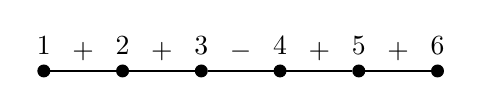
\begin{tikzpicture}[
					vertex/.style={draw, circle, inner sep=0pt, minimum size=.15cm, fill=black},
					edge/.style={thick}
					]
					% Vertices
					\node[vertex,label=above:1] (v1) at (-2,0) {};
					\node[vertex,label=above:2] (v2) at (-1,0) {};
					\node[vertex,label=above:3] (v3) at ( 0,0) {};
					\node[vertex,label=above:4] (v4) at ( 1,0) {};
					\node[vertex,label=above:5] (v5) at ( 2,0) {};
					\node[vertex,label=above:6] (v6) at ( 3,0) {};
					
					% Edges
					\draw[edge] (v1) -- node[above] {$+$} (v2);
					\draw[edge] (v2) -- node[above] {$+$} (v3);
					\draw[edge] (v3) -- node[above] {$-$} (v4);
					\draw[edge] (v4) -- node[above] {$+$} (v5);
					\draw[edge] (v5) -- node[above] {$+$} (v6);
				\end{tikzpicture}
				\caption{Signed undirected graph $ G$ of $\mathcal{P}$.}
				\label{xnfig11}
			\end{minipage}
		\end{figure}
		% This must go next to `\end{minipage}`
	be an irreducible tridiagonal sign pattern with a $0$-diagonal whose underlying signed undirected graph is $G$ given in Fig~\ref{xnfig11}. Clearly, $G$ has exactly one maximal signed path with odd length. Any real matrix $B\in \mathcal{Q}(\mathcal{P}),$ is similar to
	
	$$\begin{bmatrix}
		0&1&0&0&0&0\\ a&0&1&0&0&0\\ 0&b&0&-1&0&0\\ 0&0&c&0&1&0\\0&0&0&d&0&1\\0&0&0&0&e&0
	\end{bmatrix}, ~\text{where}~ a,b,c,d,e>0.$$
	\begin{itemize}
		\item[i.] If $a=e=\frac{1}{20}$, $b=d=5$, $c=20$ then $\sigma(B)=\{ 2.4401i, - 2.4401i, 1.9859i,- 1.9859i, 0.0461i, - 0.0461i\}$, so $\In(B)=(0,0,6)$.
		\item[ii.] If $a=b=e=d=e=1$ then $\sigma(B)=\{-1.3071 + 0.2151i, -1.3071 - 0.2151i, 1.3071 + 0.2151i, 1.3071 - 0.2151i, 0.5698i, - 0.5698i\}$, so $\In(B)=(2,2,2)$.
	\end{itemize}
	Therefore, $\mathcal{P}$ does not require a unique inertia, although it has exactly one maximal signed path with odd length.
\end{eg}

However, for irreducible tree sign patterns with a $0$-diagonal, the conclusion of Theorem~\ref{th2.51} may not hold.

\begin{eg}
	Let $\mathcal{P}$ be an irreducible tree sign pattern with a $0$-diagonal, whose underlying graph $G$ is given in Fig.~\ref{X.1}.
	\begin{figure}[H]
		\centering
		\begin{minipage}{.45\textwidth}
			\vspace{-1cm}
			\[
			\mathcal{P}=\begin{bmatrix}
				0 & - & 0 & 0 & 0 & 0 \\
				+ & 0 & + & 0 & 0 & 0 \\
				0 & + & 0 & + & 0 & + \\
				0 & 0 & + & 0 & - & 0 \\
				0 & 0 & 0 & + & 0 & 0 \\
				0 & 0 & + & 0 & 0 & 0
			\end{bmatrix}
			\]
		\end{minipage}
		\hspace{0.05\textwidth}
		\begin{minipage}{.45\textwidth}
			\centering
			\tikzset{node distance=1cm}
			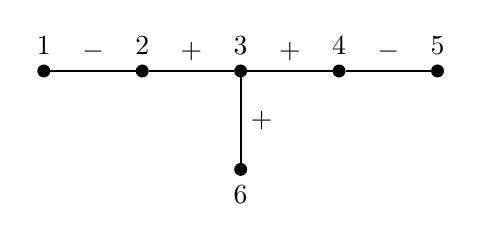
\begin{tikzpicture}[
				vertex/.style={draw, circle, inner sep=0pt, minimum size=0.15cm, fill=black},
				edge/.style={thick}
				]
				% Vertices
				\node[vertex, label=above:$1$] (v1) at (0,0) {};
				\node[vertex, label=above:$2$] (v2) at (1.25,0) {};
				\node[vertex, label=above:$3$] (v3) at (2.5,0) {};
				\node[vertex, label=above:$4$] (v4) at (3.75,0) {};
				\node[vertex, label=above:$5$] (v5) at (5,0) {};
				\node[vertex, label=below:$6$] (v6) at (2.5,-1.25) {};
				
				% Edges
				\draw[edge] (v1) -- node[above] {$-$} (v2);
				\draw[edge] (v2) -- node[above] {$+$} (v3);
				\draw[edge] (v3) -- node[above] {$+$} (v4);
				\draw[edge] (v4) -- node[above] {$-$} (v5);
				\draw[edge] (v3) -- node[right] {$+$} (v6);
			\end{tikzpicture}
			\caption{Signed undirected graph $G$ of $\mathcal{P}$.}
			\label{X.1}
		\end{minipage}
	\end{figure}
	
	Then any real matrix $B\in \mathcal{Q}(\mathcal{P})$ is similar to\\		
	$$
	\begin{bmatrix}
		0 & -a &  0&0  &0  & 0  \\
		1 & 0 & b  & 0&0 &0    \\
		0& 1 & 0  & c  & 0&e  \\
		0&0 & 1   & 0  & -d &0  \\
		0&0  &  0   & 1 & 0 & 0\\
		0&0  &  1 &  0& 0  & 0
	\end{bmatrix}\in \mathcal{Q}(\mathcal{P}),~ where~ a,b,c,d,e>0.$$
	The characteristic polynomial of $B$ is $\Ch_{B}(x)= x^6+E_2 x^4+E_4x^2+E_6$, where $E_2=a-b-c+d-e, E_4= -ac+ad-bd-ea-eb, E_6=-ead$.
	
	\textbf{Case 1:} Suppose $E_2 \geq 0$.  
	For all $x \in \mathbb{R} \setminus \{0\}$, we have
	\[
	\sgn(\Ch_{B}(x)) = 
	\begin{cases} 
		(+)+(+/0)(+)+(+/0)(+)+(-) & \text{if } E_4 \geq 0 \\[6pt]
		(+)+(+/0)(+)+(-)(+)+(-) & \text{if } E_4 < 0.
	\end{cases}
	\]
	Thus $V_+(x) = 1$ and $V_-(x) = 1$. By Descartes' rule of signs, $\Ch_B(x)$ has exactly one positive and one negative real root. Since $\det(B) \neq 0$, the eigenvalue frequency is $S_B = (2,4)$.
	
	\medskip
	
	\textbf{Case 2:} Suppose $E_2 < 0$. Then
	\begin{equation} \label{eq1}
		a - b - c + d - e < 0.
	\end{equation}
	If $E_4 \geq 0$, then
	\begin{equation} \label{eq2}
		-ac + ad - bd - ea - eb \geq 0
	\end{equation}
	\[
	\implies d \geq c+e+\left(\frac{b}{a}\right)d+\left(\frac{e}{a}\right)b 
	\;\;\implies\;\; d > c+e.
	\]
	Now, from \eqref{eq1},
	\[
	a+(d-c-e)-b < 0 \;\;\implies\;\; a < b.
	\]
	On the other hand, from \eqref{eq2},
	\[
	(a-b)d \geq ac+ea+ed > 0 \;\;\implies\;\; a > b,
	\]
	a contradiction. Therefore $E_4 < 0$.
	Hence, for all $x \in \mathbb{R} \setminus \{0\}$,
	\[
	\sgn(\Ch_{B}(x)) = (+)+(-)(+)+(-)(+)+(-).
	\]
	Thus $V_+(x) = 1$ and $V_-(x) = 1$. By Descartes' rule of signs, $\Ch_B(x)$ has exactly one positive and one negative real root. Since $\det(B) \neq 0$, the eigenvalue frequency is again $S_B = (2,4)$.
	In both cases, $S_B = (2,4)$ for all $B \in \mathcal{Q}(\mathcal{P})$, hence
	$
	S_{\mathcal{P}} = (2,4).
	$
	
	Therefore, by Corollary~\ref{c2.2}, $\mathcal{P}_-$ requires a unique inertia. However, the underlying signed undirected graph of $\mathcal{P}_-$ contains more than one maximal signed path of odd length.
\end{eg}









Next, we focus on identifying certain patterns that cannot occur as subpatterns of tridiagonal sign patterns requiring a unique inertia.
%%%%%%%%%%%%%%%%



Let, $$\mathcal{P}_4=\begin{bmatrix}
	0&+&0&0\\+&0&-&0\\0&+&0&+\\0&0&+&0
\end{bmatrix}~\text{and}~\mathcal{P}_6=\begin{bmatrix}
	0&+&0&0&0&0\\+&0&+&0&0&0\\0&+&0&-&0&0\\0&0&+&0&+&0\\0&0&0&+&0&+\\0&0&0&0&+&0
\end{bmatrix}.$$
\begin{theorem}\label{nth3.4}
	Let $\mathcal{P}\in \mathcal{Q}_n$ be an irreducible tridiagonal sign pattern with a $0$-diagonal. If $\mathcal{P}_4$ or ${\mathcal{P}_4}_-$ is a submatrix of $\mathcal{P}$, then $\mathcal{P}$ does not require a unique inertia.
\end{theorem}

In order to prove the above theorem, we first show that each of $\mathcal{P}_4$, ${\mathcal{P}_4}_-$, $\mathcal{P}_6$, ${\mathcal{P}_6}_-$ does not require a unique inertia. Also, we show that if $\mathcal{P}$ is one of the above, then there exist real matrices $B_1, B_2\in \mathcal{Q}(\mathcal{P})$ such that $\In(B_1)\neq \In(B_2)$, where both $B_1, B_2$ have all distinct eigenvalues. 
%where $\mathcal{P}$ is one of $\mathcal{P}_4$, ${\mathcal{P}_4}_-$, $\mathcal{P}_6$, ${\mathcal{P}_6}_-$.

Since each of $\mathcal{P}_4$, ${\mathcal{P}_4}_-$ has more than one maximal signed path with odd length, by Theorem \ref{th2.51}, $\mathcal{P}_4$, ${\mathcal{P}_4}_-$ does not require a unique inertia. The following example shows that there exist $B_1, B_2\in \mathcal{Q}(\mathcal{P}_4)$ such that $\In(B_1)\neq \In(B_2)$ and both $B_1, B_2$ have all distinct eigenvalues.
\begin{eg} \label{eg3.1}
	Consider $B\in \mathcal{Q}(\mathcal{P}_4),$ then $B$ is similar to
	
	$$\begin{bmatrix}
		0&1&0&0\\ a&0&-1&0\\ 0&b&0&1\\ 0&0&c&0
	\end{bmatrix},~\text{where}~ a,b,c>0.$$ Then, $\Ch_B(x)=x^4+(-a+b-c)x^2+ac$. 
	\begin{itemize}
		\item[i.] If $a=b=c=1$ then $\sigma(B_1)=\{\frac{\sqrt{3}}{2}+\frac{i}{2},\frac{\sqrt{3}}{2}- \frac{i}{2},-\frac{\sqrt{3}}{2}+ \frac{i}{2},- \frac{\sqrt{3}}{2}-\frac{i}{2}\}$, $\In(B_1)=(2,2,0)$.
		\item[ii.] If $a=1$, $b=10$ and $c=4$ then $\sigma(B_2)=\{i,-i, 2i,-2i\}$, $\In(B_2)=(0,0,4)$.
	\end{itemize}
	By Lemma \ref{3.1}, there also exists $B_1,B_2\in \mathcal{Q}({\mathcal{P}_{4}}_-)$ such that both $B_1, B_2$ have all distinct eigenvalues and $\In(B_1)\neq \In(B_2)$.
\end{eg}



\begin{eg} \label{eg2.21}
	From Example \ref{neg11}, there exists $B_1, B_2 \in \mathcal{Q}(\mathcal{P}_6)$ such that both $B_1, B_2$ have all distinct eigenvalues and
	$\In(B_1)\neq \In(B_2)$. Similarly, Lemma \ref{3.1} implies that there exists $B_1, B_2 \in \mathcal{Q}({\mathcal{P}_{6}}_-)$ such that both $B_1, B_2$ have all distinct eigenvalues and $\In(B_1)\neq \In(B_2)$.
\end{eg}





%From Example \ref{eg2.2}, there exists $B_1,B_2\in \mathcal{Q}(\mathcal{P}_{6})$ such that both $B_1, B_2$ have all distinct eigenvalues and $\In(B_1)\neq \In(B_2)$. Similarly, Lemma \ref{3.1} implies that there exists $B_1,B_2\in \mathcal{Q}(\mathcal{P}_{6_-})$ such that both $B_1, B_2$ have all distinct eigenvalues and $\In(B_1)\neq \In(B_2)$.





%\begin{proof} Suppose that $\mathcal{P}$ is an irreducible, tridiagonal sign pattern with a $0$-diagonal and $\mathcal{P}_4$ is a subpattern of $\mathcal{P}$.
%  If $n$ is an odd then $\mathcal{P}$ must contain more than one maximal signed path of odd length and by Theorem \ref{th2.5}, $\mathcal{P}$ does not require unique inertia. 

%  If $n$ is even then we prove this theorem using induction on $n$. For $n=4$, by example \ref{3.3.2}, $\mathcal{P}$ does not require unique inertia. For $n=6$, if the number of maximal signed paths of odd length is more than one then by Theorem \ref{th2.5}, $\mathcal{P}$ does not require unique inertia and if the number of maximal signed paths of odd length is at most one then by example \ref{3.5.1} $b$, $c$, $\mathcal{P}$ does not require unique inertia.

% Suppose that the statement is true for $n\leq 2k-2$ for some $k\geq 4$. For $n=2k$, if the number of maximal signed paths of odd length is more than one then by Theorem \ref{th2.5}, $\mathcal{P}$ does not require unique inertia. If the number of maximal signed paths of odd length is at most one, then suppose that $\mathcal{P}$ is an irreducible tridiagonal sign pattern with a $0$-diagonal whose underlying graph $G:v_1v_2\cdots v_{2k}$ contains $G_4:v_lv_{l+1}v_{l+2}v_{l+3}$ as a subgraph. Since $n\geq 8$, either $dist(v_1,v_l)\geq 2$ or $dist(v_{l+3},v_n)\geq 2$.  Suppose that $dist(v_1,v_l)\geq 2$ and the edges $(v_1,v_2)$, $(v_2,v_3)$ are positively signed. Consider the principal subpattern of $\mathcal{P}'$ of order $n-2$ obtained from $\mathcal{P}$ by removing the rows and columns corresponding to $v_1$ and $v_2$. Then by induction hypothesis, $\mathcal{P}'$ does not require unique inertia. 

%  Now $\gamma=(v_3,v_4)(v_5,v_6)\cdots(v_{n-1},v_n)$ is a cycle of length $n-2$ in $\mathcal{P}'$, and define the matrix $B_1(0)=(b(0)_{ij})$
%$$b(0)_{ij}= \begin{cases}
	%		1 & \text{if}\ a_{ij}=+ ~and~ is~ in~ (v_3,v_4), \\
	%		-1 & \text{if}\ a_{ij}=- ~and~ is~ in~ (v_3,v_4), \\
	%		10 & \text{if}\ a_{ij}=+ ~and~ is~ in~ (v_5,v_6), \\
	%		-10 & \text{if}\ a_{ij}=- ~and~ is~ in~ (v_5,v_6), \\
	%             \vdots\\
	%             10^{k-1} & \text{if}\ a_{ij}=+ ~and~ is~ in~ (v_{n-1},v_n), \\
	%		-10^{k-1} & \text{if}\ a_{ij}=- ~\text{and}\ is~ in~ (v_{n-1},v_n), \\
	%		0 & \text{elsewhere}
	%	\end{cases}$$ Since all eigenvalues of $B_1(0)$ are algebraically simple and eigenvalues are either real numbers or purely imaginary numbers. So for sufficiently small $\epsilon$, all eigenvalues of the perturbed matrix $B_1(\epsilon)$ are algebraically simple and eigenvalues are either real numbers or purely imaginary numbers close to the eigenvalues of $B_1(0)$. Since $\mathcal{P}'$ does not require unique inertia, so there exists a real matrix $B_2\in \mathcal{Q}(\mathcal{P}')$ with $\In(B_1(\epsilon))\neq \In(B_2)$. Suppose that 
%  $$M>max\{|\lambda|: \lambda~ is~ an~ eigenvalue~ of~either ~B_1(\epsilon)~or~B_2\},$$ 
%  and define the real matrix $$\bar{B}_1(\epsilon_1)=\begin{bmatrix}
	%      0&M&0&0&\cdots&0\\M&0&\epsilon_1&0&\cdots&0\\0&\epsilon_1&&&&\\0&0&&B_1(\epsilon)&&\\ \vdots&\vdots&&&&\\0&0&&&&
	%  \end{bmatrix}.$$
%  Then $\Bar{B}_1(\epsilon_1)\in \mathcal{Q}(\mathcal{P})$ and for small $\epsilon_1>0$, all eigenvalues of $\Bar{B}_1(\epsilon_1)$ are algebraically simple and lies close to the eigenvalues of $B_1(\epsilon)$ and $\{M,-M\}$. Similarly define $$\bar{B}_2(\epsilon_2)=\begin{bmatrix}
	%     0&M&0&0&\cdots&0\\M&0&\epsilon_2&0&\cdots&0\\0&\epsilon_2&&&&\\0&0&&B_2&&\\ %\vdots&\vdots&&&&\\0&0&&&&
	%  \end{bmatrix}.$$
%  Then $\Bar{B}_2(\epsilon_2)\in \mathcal{Q}(\mathcal{P})$ and for small $\epsilon_2>0$, all eigenvalues of $\Bar{B}_2(\epsilon_2)$ are lies close to the eigenvalues of $B_2$ and $\{M,-M\}$. Since $\In(B_1(\epsilon))\neq \In(B_2)$, therefore for sufficiently small $\epsilon_1$ and $\epsilon_2$, $\In(\bar{B}_1(\epsilon_1))\neq \In(\bar{B}_2(\epsilon_2))$. Hence $\mathcal{P}$ does not require unique inertia.
%\end{proof}

\begin{proof}[Proof of Theorem \ref{nth3.4}]
	Suppose that $\mathcal{P}=[p_{ij}]\in \mathcal{Q}_n$ is an irreducible tridiagonal sign pattern with a $0$-diagonal such that $\mathcal{P}_4$ is a submatrix of $\mathcal{P}$, then $n\geq 4$. Let $G$ be the signed undirected graph corresponding to $\mathcal{P}$. If the number of maximal signed paths of odd length in $G$ is more than one, then by Theorem \ref{th2.51}, $\mathcal{P}$ does not require a unique inertia, so we assume that the number of maximal odd length paths in $G$ is exactly one, which implies that $n$ is even.
	
	% Let $G$ be the signed undirected graph corresponding to $\mathcal{P}$.
	%If $n$ is odd, then $G$ must contain more than one maximal signed path of odd length, so by Theorem \ref{th2.51}, $\mathcal{P}$ does not require a unique inertia.
	
	For $n=4$, by Example \ref{eg3.1}, $\mathcal{P}$ does not require a unique inertia. For $n=6$, since the number of maximal signed paths of odd length in $G$ is at most one, $\mathcal{P}$ is equivalent to $\mathcal{P}_6$, so by Example \ref{eg2.21}, $\mathcal{P}$ does not require a unique inertia. 
	
	For $n=2k$ with $k\geq4$, the underlying signed directed graph of $\mathcal{P}$ is given by $D = \alpha_1\alpha_2\cdots \alpha_{n-1}$, where each $\alpha_i = p_{i,i+1}p_{i+1,i}$ for $i = 1, 2, \dots, n-1$ represents a $2$-cycle in $D$. Let $D_4 = \alpha_l\alpha_{l+1}\alpha_{l+2}$ be the subgraph of $D$, which is the signed directed graph corresponding to $\mathcal{P}_4$. %and $G_6=(v_{l-1},v_l),(v_l,v_{l+1}),(v_{l+1},v_{l+2}),(v_{l+2},v_{l+3}),(v_{l+3},v_{l+4})$ as subgraphs.
	Since the number of maximal signed paths of odd length in $G$ is one, $D_6=\alpha_{l-1}\alpha_{l}\alpha_{l+1}\alpha_{l+2}\alpha_{l+3}$ is also a subgraph of $D$, which is the signed directed graph corresponding to $\mathcal{P}_6$ and
	$$\gamma=\alpha_1\alpha_3\cdots\alpha_{l-3}\alpha_{l+5}\cdots\alpha_{n-1},$$ is a composite cycle in $D\setminus V(D_6)$ of length $n-6$.% consisting only of $2$-cycles.
	
	
	From Example \ref{eg2.21}, there exist two real matrices $B_1=[(b_1)_{ij}]$, $B_2=[(b_2)_{ij}]$ in $\mathcal{Q}(\mathcal{P}_6)$ with $\In(B_1)\neq \In(B_2)$ such that both $B_1, B_2$ have all distinct eigenvalues. Let,
	$$M>\max\{1,|\lambda|: \lambda~ \text{is}~ \text{an}~ \text{eigenvalue}~ \text{of}~\text{either} ~B_1~\text{or}~B_2\}$$ and define the real matrices $B_{r,\gamma}(0)=[b_{r,\gamma}(0)_{ij}]$ for $r=1,2$, as
	$$(b_{r,\gamma}(0))_{ij}= \begin{cases}
		M^p & \text{if}\ p_{ij}=+~\text{and}~ \text{is}~ \text{in}~ \alpha_p,~\text{for}~p=1,3,...,l-3,l+5,...,n-1 \\
		-M^p & \text{if}\ p_{ij}=-~\text{and}~ \text{is}~ \text{in}~ \alpha_p,~\text{for}~p=1,3,...,l-3,l+5,...,n-1 \\
		
		(b_{r})_{i+2-l,j+2-l} & \text{if}\ l-1\leq i,j\leq l+4 \\
		
		0 & \text{elsewhere.}
	\end{cases}$$
	Then the eigenvalues of $B_{1,\gamma}(0)$, $B_{2,\gamma}(0)$ are algebraically simple and the eigenvalues of $B_{r,\gamma}(0)$, $r=1,2$ are the eigenvalues of $B_r$ together with the second complex roots of $M^{2p}$ or $-M^{2p}$, depending on the sign of $\alpha_p$, for $p=1,3,...,l-3,l+5,...,n-1$. Note that both $B_{1,\gamma}(0)$, $B_{2,\gamma}(0)$ have all distinct eigenvalues and $\In(B_{1,\gamma}(0))\neq \In(B_{2,\gamma}(0))$. For $\epsilon>0$ define the perturbed matrices $B_{r,\gamma}(\epsilon)=[b_{r,\gamma}(\epsilon)_{ij}]$ for $r=1,2$, as
	\[
	(b_{r,\gamma}(\epsilon))_{ij} = 
	\begin{cases}
		(b_{r,\gamma}(0))_{ij} & \text{if } p_{ij} \neq 0 \text{ and } (b_{r,\gamma}(0))_{ij} \neq 0 \\
		\epsilon & \text{if } p_{ij} = + \text{ and } (b_{r,\gamma}(0))_{ij} = 0 \\
		-\epsilon & \text{if } p_{ij} = - \text{ and } (b_{r,\gamma}(0))_{ij} = 0 \\
		0 & \text{otherwise.}
	\end{cases}
	\]
	Then $B_{1,\gamma}(\epsilon),B_{2,\gamma}({\epsilon})\in \mathcal{Q}(\mathcal{P})$. For $\epsilon>0$ sufficiently small, all the eigenvalues of $B_{1,\gamma}(\epsilon)$ remain close to the eigenvalues of $B_{1,\gamma}(0)$.   The eigenvalues of $B_{1,\gamma}(\epsilon)$ close to the real eigenvalues of $B_{1,\gamma}(0)$ of the form $\lambda$, $-\lambda$ must be real and of the same form, since they cannot merge to form conjugate pairs of nonreal eigenvalues. Similarly, the eigenvalues of $B_{1,\gamma}(\epsilon)$ close to the nonreal eigenvalues of $B_{1,\gamma}(0)$ of the form $i\lambda$, $-i\lambda$ must be nonreal and of the same form. Therefore, for $\epsilon>0$, sufficiently small, $\In(B_{1,\gamma}(0))=\In(B_{1,\gamma}(\epsilon))$.
	
	%Since $B_{1,\gamma}(0)$ has all distinct eigenvalues by repeating the argument as in the proof of Theorem \ref{l3.1n}, it can be shown that $\In(B_{1,\gamma}(0))=\In(B_{1,\gamma}(\epsilon))$ for $\epsilon>0$ is sufficiently small.
	Similarly, since $B_{2,\gamma}(0)$ has all distinct eigenvalues, there exists $\bar{\epsilon}>0$ sufficiently small such that $\In(B_{2,\gamma}(0))=\In(B_{2,\gamma}(\bar{\epsilon}))$. Since $\In(B_{1,\gamma}(0))\neq \In(B_{2,\gamma}(0))$, $\In(B_{1,\gamma}(\epsilon))\neq \In(B_{2, \gamma}(\bar{\epsilon}))$ therefore, $\mathcal{P}$ does not require a unique inertia.
	
	Similarly, if $\mathcal{P}_{4-}$ is a submatrix of $\mathcal{P}$, then it can be shown that $\mathcal{P}$ does not require a unique inertia.
\end{proof}
%Then $D_i\cap D_j=\phi$ whenever $\lambda_i\neq\lambda_j$. Eigenvalues of $B_{1,\gamma_1}(0)$ are algebraically simple and the eigenvalues of $B_{1,\gamma_1}(\epsilon)$ are continuous functions of $\epsilon$, so for sufficiently small $\epsilon>0$, each $D_i$ contain exactly one eigenvalue of $B_{1,\gamma_1}(\epsilon)$. Suppose that $\lambda_j=a_j+ib_j$ for $j=1,2,...,n$ is an eigen value of $B_{1,\gamma_1}(\epsilon)$, if $a_j\neq0$ then $D_j$ does not intersects imaginary axis and if $b_j\neq 0$ then $D_j$ does not intersects real axis, we conclude that $\In(B_{1,\gamma_1}(0))=\In(B_{1,\gamma_1}(\epsilon))$. Similarly, for $r=2$, there exists some small $\bar{\epsilon}>0$ such that $\In(B_{2,\gamma_1}(0))=\In(B_{2,\gamma_1}(\bar{\epsilon}))$.  Since $B_{1,\gamma_1}(\epsilon),B_{2,\gamma_1}(\bar{\epsilon})\in \mathcal{Q}(\mathcal{P})$ and $\In(B_1)\neq \In(B_2)$, therefore $\In(B_{1,\gamma_1}(\epsilon))\neq \In(B_{2, \gamma_1}(\bar{\epsilon}))$. Hence $\mathcal{P}$ does not require a unique inertia.
%$$|(b_r(\epsilon))_{ij}|= \begin{cases}
	%		M & \text{if}\ a_{ij}~ is~ in~ (v_1,v_2), \\
	%		M^3 & \text{if}\ a_{ij}~ is~ in~ (v_3,v_4), \\
	%           \vdots\\
	%		M^{l-2} & \text{if}\ a_{ij}~is~ in~ (v_{l-2},v_{l-1}), \\
	%  M^{l+4} & \text{if}\ a_{ij}~is~ in~ (v_{l+4},v_{l+5}), \\
	%  \vdots\\
	%  M^{n-1} & \text{if}\ a_{ij}~is~ in~ (v_{n-1},v_{n}), \\
	
	%		|b_r|_{i+1-l,j+1-l} & \text{if}\ l\leq i,j\leq l+3, \\
	%    \epsilon & \text{if}\ a_{ij}\neq0~not~in~\gamma_1~and~either~1\leq i,j\leq l~or~l+3\leq i,j\leq n\\
	%   0 & \text{elsewhere.}
	%	\end{cases}$$
% Then for $r=1,2$, $B_{\gamma_1}^r(\epsilon)\in \mathcal{Q}(\mathcal{P})$ and for small $\epsilon>0$, all eigenvalues of $B_{\gamma_1}^r(\epsilon)$ are lies close to the eigenvalues of $B_r$ and $M^p,-M^p$ or $iM^p,-iM^p$ depending upon the sign of the cycle $(v_p,v_{p+1})$ for $p=1,3,...,l-2,l+4,...,n-1$. Since $\In(B_1)\neq \In(B_2)$ and both $B_1, B_2$ have all distinct eigenvalues, therefore for sufficiently small $\epsilon>0$, $\In(B_{\gamma_1}^1(\epsilon))\neq \In(B_{\gamma_1}^2(\epsilon))$. Hence $\mathcal{P}$ does not require unique inertia. 
%	If $\text{dist}(1,l)$ is odd, then $\mathcal{P}_6$ is a subpattern of $\mathcal{P}$. By considering $B_1, B_2\in \mathcal{Q}(\mathcal{P}_6)$ such that both $B_1, B_2$ has all distinct eigenvalues and $\In(B_1)\neq \In(B_2)$ it can be similarly shown that  $\mathcal{P}$ does not require a unique inertia.









When the order of $\mathcal{P}$ is greater than or equal to $6$, we specify another pattern which also cannot be a subpattern of a tridiagonal sign pattern requiring a unique inertia.





Let, $$\mathcal{P}_6'=\begin{bmatrix}
	0&+&0&0&0&0\\+&0&-&0&0&0\\0&+&0&-&0&0\\0&0&+&0&-&0\\0&0&0&+&0&+\\0&0&0&0&+&0
\end{bmatrix}, ~~~
\mathcal{P}_8'=\begin{bmatrix}
	0&+&0&0&0&0&0&0\\+&0&+&0&0&0&0&0\\0&+&0&-&0&0&0&0\\0&0&+&0&-&0&0&0\\0&0&0&+&0&-&0&0\\0&0&0&0&+&0&+&0\\0&0&0&0&0&+&0&+\\0&0&0&0&0&0&+&0
\end{bmatrix}.$$
The following examples show that there exists $B_1, B_2\in \mathcal{Q}(\mathcal{P}_6')$ (or, $\mathcal{Q}(\mathcal{P}_8'$)) such that both $B_1,B_2$ have all distinct eigenvalues and $\In(B_1)\neq \In(B_2)$, which implies, $\mathcal{P}_6'$ (or, $\mathcal{P}_8'$) does not require a unique inertia.

\begin{eg} \label{ega21} 
	Take $B\in \mathcal{Q}(\mathcal{P}_6'),$ then $B$ is similar to
	
	$$\begin{bmatrix}
		0&1&0&0&0&0\\a&0&-1&0&0&0\\0&b&0&-1&0&0\\0&0&c&0&-1&0\\0&0&0&d&0&1\\0&0&0&0&e&0
	\end{bmatrix}, ~\text{where}~ a,b,c,d,e>0.$$ \\
	
	\begin{itemize}
		\item[i.] If $B_1\in \mathcal{Q}(\mathcal{P}_6')$ is such that $a=10$, $b=c=d=e=1$, then $\sigma(B_1)=\{-3.0148,  3.0148, 0.7983, -0.7983, 1.3139i, -1, 3139i\}$, so $In(B_1)=(2,2,2)$ and $B_1$ has all distinct eigenvalues. 
		\item[ii.] If $B_2\in \mathcal{Q}(\mathcal{P}_6')$ is such that $a=e=\frac{1}{20}$, $b=d=5$, $c=20$, then $\sigma(B_2)=\{ 5.3970i,-5.3970i, 0.8776i, -0.8776i, 0.0472i, 0.0472i\}$, so $In(B_2)=(0,0,6)$ and $B_2$ has all distinct eigenvalues.
	\end{itemize}
	%Therefore, $\mathcal{P}'$ does not require a unique inertia.
\end{eg}

\begin{eg}\label{ega11}  Take $B\in \mathcal{Q}(\mathcal{P}_8'),$ then $B$ is similar to
	$$\begin{bmatrix}
		0&1&0&0&0&0&0&0\\a&0&1&0&0&0&0&0\\0&b&0&-1&0&0&0&0\\0&0&c&0&-1&0&0&0\\0&0&0&d&0&-1&0&0\\0&0&0&0&e&0&1&0\\0&0&0&0&0&f&0&1\\0&0&0&0&0&0&g&0
	\end{bmatrix},~\text{where}~ a,b,c,d,e,f,g,h>0.$$ 
	
	\begin{itemize}
		\item[i.] If $B_1\in \mathcal{Q}(\mathcal{P}_8')$ is such that $a=b=c=d=e=f=g=1$ then $\sigma(B_1)=\{-1.3096 + 0.0611i, -1.3096 - 0.0611i, 1.3096 + 0.0611i, 1.3096 - 0.0611i, 1.5080i, - 1.5080i,  -0.3858i,0.3858i\}$, so $In(B_1)=(2,2,4)$ and $B_1$ has all distinct eigenvalues.
		%\item[ii.] If $B_2\in \mathcal{Q}(\mathcal{P}_8')$ is such that $a=10$, $b=c=d=e=f=g=1$ then $\sigma(B_2)=\{-3.3049, 3.3049,\\-1.3047,1.3047,-1.5493i, 1.5493i,-0.4734i, 0.4734i\}$, so $In(B_2)=(2,2,4)$ and 
		\item[ii.] If $B_2\in \mathcal{Q}(\mathcal{P}_8')$ is such that $a=g=\frac{1}{20}$, $b=d=f=5$, $c=e=20$ then $\sigma(B_2)=\{ 5.3989i,-5.3989i, 2.2575i, -2,2575i, 0.1022i,-0.1022i,0.8032i,0.8032i\}$, so $In(B_2)=(0,0,8)$ and $B_2$ has all distinct eigenvalues.
	\end{itemize}
	%Therefore, $\mathcal{P}_8'$ does not require a unique inertia.
\end{eg}

\begin{theorem}\label{nth8} \label{nth3.18}
	Let $\mathcal{P}\in \mathcal{Q}_n$ be an irreducible tridiagonal sign pattern with a $0$-diagonal. If $\mathcal{P}_6'$ or ${\mathcal{P}_6'}_-$ is a submatrix of $\mathcal{P}$, then $\mathcal{P}$ does not require a unique inertia.
\end{theorem}

\begin{proof}
	Suppose that $\mathcal{P}=[p_{ij}]\in \mathcal{Q}_n$ is an irreducible tridiagonal sign pattern with a $0$-diagonal such that $\mathcal{P}_6'$ is a submatrix of $\mathcal{P}$, thus $n\geq 6$. Let $G$ be the signed undirected graph corresponding to $\mathcal{P}$. If the number of maximal signed paths of odd length in $G$ is more than one, then by Theorem \ref{th2.51}, $\mathcal{P}$ does not require a unique inertia, so we assume that the number of maximal odd length paths in $G$ is exactly one, which implies that $n$ is even.
	%$\mathcal{P}$ does not require a unique inertia.
	%So we assume 
	%	If $n$ is odd, then $G$ must contain more than one maximal signed path of odd length, so by Theorem \ref{th2.51}, $\mathcal{P}$ does not require a unique inertia. 
	
	For $n=6$, by Example \ref{ega21}, $\mathcal{P}$ does not require a unique inertia. For $n=8$, since the number of maximal signed paths of odd length in $G$ is one, $\mathcal{P}$ is equivalent to $\mathcal{P}_8'$. By Example \ref{ega11}, $\mathcal{P}$ does not require a unique inertia, and there exists $B_1, B_2\in \mathcal{Q}(\mathcal{P})$ such that $\In(B_1)\neq \In(B_2)$ and both $B_1, B_2$ have all distinct eigenvalues.
	
	For $n=2k$ with $k\geq5$, since the number of maximal signed paths of odd length in $G$ is one, $\mathcal{P}_8'$ is a submatrix of $\mathcal{P}$ and by proceeding as in Theorem \ref{nth3.4}, it can be shown that $\mathcal{P}$ does not require a unique inertia.
	
	Similarly, if ${\mathcal{P}_{6-}'}$ is a submatrix of $\mathcal{P}$, then $\mathcal{P}$ does not require a unique inertia.
\end{proof} 


%%%%%%%%%%%%%%%%%%%%%%%%%%%%%%%%%%%%%%%%%%%%%%%%%%%%%%%%%%%%%%%%%%%%%%%%%%%%%%%%%%%%%%%%%%




\section{Combinatorially symmetric sign patterns with underlying graphs containing cycles, which require a unique inertia} \label{s4}

In this section, we focus on irreducible combinatorially symmetric sign patterns, where the underlying undirected graphs contain cycles but no loops. Interesting and easily verifiable necessary conditions are obtained for such patterns to require a unique inertia, depending on the signs of the edges, the distances between cycles, and the distances from leaves to cycles in the underlying graph.

\begin{theorem}\label{nth0.11}
	Let $\mathcal{P}\in \mathcal{Q}_n$, where $n$ is odd, be an irreducible combinatorially symmetric sign pattern with a $0$-diagonal whose underlying signed undirected graph is a cycle. Then the following is true.
	\begin{itemize}
		\item[i.] If $\mathcal{P}$ allows singularity, then $\mathcal{P}$ does not require a unique inertia.
		\item[ii.] If $\mathcal{P}$ is sign nonsingular, then $\mathcal{P}$ requires a unique inertia. 
	\end{itemize}
\end{theorem}
\begin{proof}
	\begin{itemize}
		\item[i.] If $\mathcal{P}$ allows singularity, and since $\mathcal{P}$ is not sign singular, then there exist two composite cycles $\Gamma_1$, $\Gamma_2$ of length $n$ in the underlying signed directed graph of $\mathcal{P}$ such that $\sgn(\Gamma_1) = -\sgn(\Gamma_2)$.
		% $A_+,A_- \in \mathcal{Q}(\mathcal{P})$ with $\det(A_+)>0$ and $\det(A_-)<0$. 
		Hence, by Lemma~\ref{xnl1}, $\mathcal{P}$ does not require a unique inertia.
		\item[ii.] If $\mathcal{P}$ is sign nonsingular, then for any $B\in \mathcal{Q}(\mathcal{P})$, the characteristic polynomial of $B$ has the form $$\Ch_B(x)=x^n+E_2(B)x^{n-2}+\cdots+E_{n-1}(B)x+(-1)^nE_n(B),$$ where $E_n(B)\neq 0$. Since the only non-vanishing term of even power of $x$ in $\Ch_B(x)$ is $E_n(B)~(\neq 0)$, $i\lambda$ is not a root of $\Ch_B(x)=0$ for any $\lambda\in\mathbb{R}$, so $B$ has no eigenvalues with zero real part. Hence, by Theorem \ref{th4}, $\mathcal{P}$ requires a unique inertia.
	\end{itemize}
\end{proof}

\begin{eg}\label{xxeg1}
	Suppose that $\mathcal{P}\in \mathcal{Q}_3$ is an irreducible combinatorially symmetric sign pattern with a $0$-diagonal, whose underlying signed undirected graph $G$ is given in Fig.~\ref{xx1}.
	\begin{figure}[H]
		\centering
		\begin{minipage}{.45\textwidth}
			\vspace{-1cm}
			\[
			\mathcal{P}=
			\begin{bmatrix}
				0 & + & + \\
				+ & 0 & + \\
				- & + & 0
			\end{bmatrix}
			\]
		\end{minipage}
		\hspace{0.05\textwidth}
		\begin{minipage}{.45\textwidth}
			\centering
			\tikzset{node distance=1cm}
			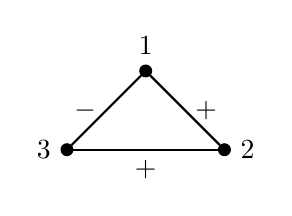
\begin{tikzpicture}[
				vertex/.style={draw, circle, inner sep=0pt, minimum size=.15cm, fill=black},
				edge/.style={thick}
				]
				% Vertices
				\node[vertex,label=left:3]  (v1) at(-1,0) {};
				\node[vertex,label=right:2] (v2) at( 1,0) {};
				\node[vertex,label=above:1] (v3) at( 0,1) {};
				
				% Edges
				\draw[edge] (v1)--node[below]{$+$}(v2);
				\draw[edge] (v2)--node[right]{$+$}(v3);
				\draw[edge] (v3)--node[left] {$-$}(v1);
			\end{tikzpicture}
			\caption{ $G$.}
			\label{xx1}
		\end{minipage}
	\end{figure}
	
	Then $\Gamma_1 = p_{12}p_{23}p_{31}$ and $\Gamma_2 = p_{13}p_{32}p_{21}$ are two oppositely signed cycles of length $3$ in the signed directed graph of $\mathcal{P}$. Hence, $\mathcal{P}$ allows singularity. Therefore, $\mathcal{P}$ satisfies the conditions stated in (i) of Theorem~\ref{nth0.11}, which implies that $\mathcal{P}$  does not require a unique inertia.
\end{eg}
\begin{eg}
	Consider an irreducible combinatorially symmetric sign pattern $\mathcal{P}\in \mathcal{Q}_3$ with a $0$-diagonal whose underlying signed undirected graph $G$ is given in Fig.~\ref{xx2}.
	\begin{figure}[H]
		\centering
		\begin{minipage}{.45\textwidth}
			\vspace{-1cm}
			\[
			\mathcal{P}=
			\begin{bmatrix}
				0 & + & + \\
				+ & 0 & + \\
				+ & + & 0
			\end{bmatrix}
			\]
		\end{minipage}
		\hspace{0.05\textwidth}
		\begin{minipage}{.45\textwidth}
			\centering
			\tikzset{node distance=1cm}
			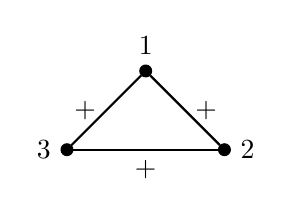
\begin{tikzpicture}[
				vertex/.style={draw, circle, inner sep=0pt, minimum size=.15cm, fill=black},
				edge/.style={thick}
				]
				% Vertices
				\node[vertex,label=left:3]  (v1) at(-1,0) {};
				\node[vertex,label=right:2] (v2) at( 1,0) {};
				\node[vertex,label=above:1] (v3) at( 0,1) {};
				
				% Edges
				\draw[edge] (v1)--node[below]{$+$}(v2);
				\draw[edge] (v2)--node[right]{$+$}(v3);
				\draw[edge] (v3)--node[left] {$+$}(v1);
			\end{tikzpicture}
			\caption{$G$}
			\label{xx2}
		\end{minipage}
	\end{figure}
	
	Then $\Gamma_1 = p_{12}p_{23}p_{31}$ and $\Gamma_2 = p_{13}p_{32}p_{21}$ are the only composite cycles of length $3$ in the signed directed graph of $\mathcal{P}$, and they have the same sign. Hence, $\mathcal{P}$ is sign nonsingular. Therefore, $\mathcal{P}$ satisfies the conditions stated in (ii) of Theorem~\ref{nth0.11}, which implies that $\mathcal{P}$ requires a unique inertia.
\end{eg}


\begin{lemma}\label{xnl2}
	Let $\mathcal{P} \in \mathcal{Q}_n$ be a sign pattern, whose underlying signed directed graph $D$ contain only cycles of even length. Suppose that the maximum length of the composite cycles in $D$ is $m$, $m \geq 2$. If $D$ contains two composite cycles, $\Gamma_1$, $\Gamma_2$, consisting only of negative $2$-cycles and positive $2$-cycles, respectively, and if $l(\Gamma_1)+l(\Gamma_2)\geq m+2$, then $\mathcal{P}$ does not require a unique inertia.
\end{lemma}
\begin{proof}
	Let $\Gamma_1 = \alpha_{i_1} \alpha_{i_2} \cdots \alpha_{i_{k_1}}$ and $\Gamma_2 = \alpha_{j_1} \alpha_{j_2} \cdots \alpha_{j_{k_2}}$ be two composite cycles in $D$ such that $\Gamma_1$ consists only of negative $2$-cycles and $\Gamma_2$ consists only of positive $2$-cycles, with $l(\Gamma_1)+l(\Gamma_2)=2k_1+2k_2\geq m+2$, where each $\alpha_t$ denotes a $2$-cycle.   Define the real matrix $B_{\Gamma_1}(0)=[b_{\Gamma_1}(0)_{ij}]$ as
	$$b_{\Gamma_1}(0)_{ij}= \begin{cases}
		10^p & \text{if}\ p_{ij}=+~\text{and}~ \text{is}~
		\text{in}~ \alpha_p,~\text{for}~p=i_1,i_2,...,i_{k_1} \\
		-10^p & \text{if}\ p_{ij}=-~\text{and}~ \text{is}~ \text{in}~ \alpha_p,~\text{for}~p=i_1,i_2,...,i_{k_1} \\
		
		0 & \text{elsewhere.}
	\end{cases}$$
	Then the eigenvalues of $B_{\Gamma_1}(0)$ are the second complex roots of $-10^{2p}$ for $p=i_1,i_2,...,i_{k_1}$. Therefore, %$B_{\gamma_1}(0)$ as in Theorem \ref{nth1}, then 
	$B_{\Gamma_1}(0)$ has $2k_1$ algebraically simple nonzero purely imaginary eigenvalues. For $\epsilon>0$, sufficiently small define $B_{\Gamma_1}(\epsilon)$ as in \eqref{e2} with $\gamma$ replaced by $\Gamma_1$, then $B_{\Gamma_1}(\epsilon)\in \mathcal{Q}(\mathcal{P})$ and its eigenvalues remain close to the eigenvalues of $B_{\Gamma_1}(0)$. Also, $D$ contains only cycles of even length, so the characteristic polynomial $\Ch_{B_{\Gamma_1}(\epsilon)}(x)$ consists only of even powers of $x$, so by Lemma \ref{lem1}, $i_0(B_{\Gamma_1}(\epsilon))\geq (n-m)+2k_1$.
	
	Similarly, define the real matrix $B_{\Gamma_2}(0)$, then it has $2k_2$ algebraically simple, nonzero real eigenvalues. For $\epsilon'>0$, sufficiently small define $B_{\Gamma_2}(\epsilon')$ as in \eqref{e2} with $\gamma$ replaced by $\Gamma_2$, then $B_{\Gamma_2}(\epsilon')\in \mathcal{Q}(\mathcal{P})$ and the eigenvalues are remain close to the eigenvalues of $B_{\Gamma_2}(0)$. So, $n-i_0(B_{\Gamma_2}(\epsilon'))\geq 2k_2$, and $$i_0(B_{\Gamma_1}(\epsilon))+(n-i_0(B_{\Gamma_2}(\epsilon')))\geq (n-m)+2k_1+2k_2\geq n+2.$$ Hence, by Theorem \ref{lem2}, $\mathcal{P}$ does not require a unique inertia.
\end{proof}

\begin{theorem} \label{xxth3}
	Let $\mathcal{P} \in \mathcal{Q}_n$ be an irreducible combinatorially symmetric sign pattern with a $0$-diagonal, whose underlying signed undirected graph $G$ is a cycle. Then $\mathcal{P}$ does not require a unique inertia if any one of the following holds:
	\begin{itemize}
		\item[i.] $G$ has an odd number of negative edges. 
		\item[ii.] Every edge of $G$ is negative.
		\item[iii.] $n$ is even and $G$ has a maximal signed path of odd length.
	\end{itemize}
\end{theorem}

\begin{proof}
	Let $D$ be the underlying signed directed graph of $\mathcal{P}$.
	\begin{itemize}
		\item[i.]  If $G$ contains an odd number of negative edges, then
		$$p_{12}p_{23}\cdots p_{n-1,n} p_{n1}=-p_{1n}p_{n,n-1}\cdots p_{32} p_{21},$$ where $p_{ij}$ is the $(i,j)$-th entry of $\mathcal{P}$.
		Let $\Gamma_1 = p_{12}p_{23}\cdots p_{n-1,n} p_{n1}$, $\Gamma_2 = p_{1n}p_{n,n-1}\cdots p_{32} p_{21}$.
		Then $\Gamma_1$, $\Gamma_2$ are two oppositely signed cycles in $D$ of length $n$, so by Lemma~\ref{xnl1}, $\mathcal{P}$ does not require a unique inertia.
		
		\item[ii.] If $n$ is odd and all edges are negatively signed, then by part~(i), $\mathcal{P}$ does not require a unique inertia. Therefore, suppose that $n$ is even. Let 
		$\Gamma_1=(1,2)(3,4)\cdots (n-1,n)$, $\Gamma_2=(1,2,...,n)$ be two composite cycles in $D$, each of length $n$.  
		Define a real matrix $B_{\Gamma_1}(\epsilon) = [b_{\Gamma_1}(\epsilon)_{ij}] \in \mathcal{Q}(\mathcal{P})$ by
		\begin{equation*}
			|b_{\Gamma_1}(\epsilon)_{ij}|= \begin{cases}
				10^p & \text{if}\ p_{ij}\neq 0 ~\text{and~is~in}~ (p,p+1),~\text{for}~p=1,3,...,n-1 \\
				\epsilon & \text{if}\ p_{ij}\neq 0~\text{and~not~in}~ \Gamma_1 \\
				
				0 & \text{elsewhere,}
			\end{cases}
		\end{equation*}
		for some $\epsilon>0$. Then $B_{\Gamma_1}(\epsilon)$ is a real skew-symmetric matrix, and hence $\In(B_{\Gamma_1}(\epsilon))=(0,0,n)$. Also, define two real matrices $B_{\Gamma_2}(0)$ and $B_{\Gamma_2}(\epsilon)$ as in \eqref{e1} and \eqref{e2}, respectively, with $\gamma$ replaced by $\Gamma_2$. Since $B_{\Gamma_2}(0)$ has $n$ nonzero algebraically simple eigenvalues, which are the $n$-th complex roots of $+1$ or $-1$ $(n\geq 3)$, it follows that for $\epsilon > 0$ sufficiently small, $B_{\Gamma_2}(\epsilon)\in \mathcal{Q}(\mathcal{P})$ and it has $n$ nonzero algebraically simple eigenvalues close to those of $B_{\Gamma_2}(0)$. Therefore, $\In(B_{\Gamma_2}(\epsilon))\neq (0,0,n)$, and $\mathcal{P}$ does not require a unique inertia. 
		
		\item[iii.] Suppose that $n$ is even and $G$ has a maximal signed path of odd length. Without loss of generality, let $P=\{1,2\}\{2,3\}\cdots\{2p-1,2p\}$ be the maximal signed path in $G$ of odd length. Since $n$ is even, the path from $2p$ to $1$ is of odd length.
		Consider,
		$$\Gamma=\{\{2j-1,2j\}: 1\leq j \leq p\}~\cup~\{\{2i,2i+1\}:2p\leq 2i\leq (n-2)\}~\cup~\{\{n,1\}\}. $$ 
		\begin{figure}[H]
			\tikzset{node distance=1cm}
			\centering
			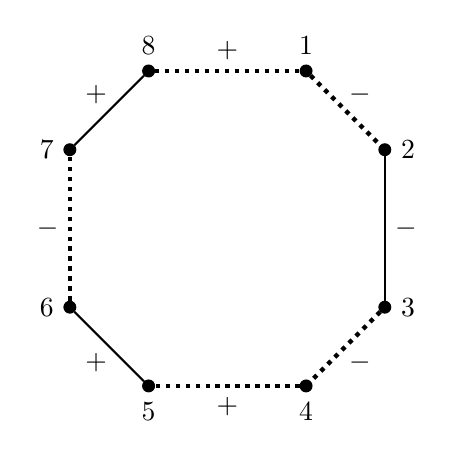
\begin{tikzpicture}
				\tikzstyle{vertex}=[draw, circle, inner sep=0pt, minimum size=.15cm, fill=black]
				\tikzstyle{edge}=[,thick]
				\node[vertex,label=above:1](v1)at(1,2){};
				\node[vertex,label=right:2](v2)at(2,1){};
				\node[vertex,label=right:3](v3)at(2,-1){};
				\node[vertex,label=below:4](v4)at(1,-2){};
				\node[vertex,label=below:5](v5)at(-1,-2){};
				\node[vertex,label=left:6](v6)at(-2,-1){};
				\node[vertex,label=left:7](v7)at(-2,1){};
				\node[vertex,label=above:8](v8)at(-1,2){};
				%\node[vertex,label=center:1](v9)at(12,0){};
				\draw[edge, ultra thick, dotted](v1)--node[right, yshift=0.2cm, xshift=-0.1cm]{$-$}(v2);
				\draw[edge](v2)--node[right]{$- $}(v3);
				\draw[edge, ultra thick, dotted](v3)--node[right, yshift=-0.2cm, xshift=-0.1cm]{$-$}(v4);
				\draw[edge, ultra thick, dotted](v4)--node[below]{$+$}(v5);
				\draw[edge](v5)--node[left, yshift=-0.2cm, xshift=0.1cm]{$+$}(v6);
				\draw[edge, ultra thick, dotted](v6)--node[left]{$-$}(v7);
				\draw[edge](v7)--node[left, yshift=0.2cm, xshift=0.1cm]{$ +$}(v8);
				\draw[edge, ultra thick, dotted](v8)--node[above]{$+$}(v1);
			\end{tikzpicture}\caption{ In the above figure $G$ is a cycle of length $8$ and $P=\{1,2\}\{2,3\}\{3,4\}$, where the dotted edges correspond to $\Gamma$.} \end{figure}
		Then the edges $\{2p-1,2p\}$, $\{2p,2p+1\}$; $\{n,1\}$, $\{1,2\}$ are the only pair of edges in $\Gamma$ which are adjacent, and the edges in each pair are signed oppositely. Hence, the positive edges in $\Gamma$, the negative edges in $\Gamma$ are all non-adjacent. Let $k_1$ (respectively, $k_2$) be the number of negative (respectively, positive) edges in $\Gamma$. Since every vertex of $G$ occurs once in $\Gamma$ except $2p$, $1$, which occurs twice, hence $2k_1+2k_2=n+2$. 
		Let $\mathcal{M}_1=\{\alpha_{i_1},\alpha_{i_2},..., \alpha_{i_{k_1}}\}$ and $\mathcal{M}_2=\{\alpha_{j_1},\alpha_{j_2},..., \alpha_{j_{k_2}}\}$ be two matchings in $G$ containing only negative and positive edges in $\Gamma$, respectively, where $\alpha_t=\{t,t+1\}$ for $t=1,2,...,n-1$, and $\alpha_n=\{n,1\}$. 
		
		Let $\Gamma_1$, $\Gamma_2$ be the composite cycles in $D$ corresponding to $\mathcal{M}_1$, $\mathcal{M}_2$, respectively. Then, $\Gamma_1$ (respectively, $\Gamma_2$) consisting only of negative (respectively, positive) $2$-cycles of $D$, and since $l(\Gamma_1) + l(\Gamma_2) = n + 2$, it follows from Lemma~\ref{xnl2} that $\mathcal{P}$ does not require a unique inertia. 
	\end{itemize} 
\end{proof}

%\begin{eg}
%    Let $\mathcal{P}\in \mathcal{Q}_3$ be an irreducible combinatorially symmetric sign pattern with a $0$-diagonal, whose underlying undirected graph $G$ is given in Example~\ref{xxeg1}.
% Then $G$ is a cycle of length $3$, which contains exactly one negative edge. Thus, $\mathcal{P}$ satisfies the conditions stated in Theorem~\ref{xxth3}(i), and, consequently, $\mathcal{P}$ does not require a unique inertia.
%\end{eg}

The following example shows that if $\mathcal{P}$ does not satisfy any of the three conditions of the previous theorem, then we cannot conclude either way, that is, in that case, $\mathcal{P}$ may or may not require a unique inertia.

\begin{eg}\label{eg0.6}
	Suppose that $\mathcal{P}\in \mathcal{Q}_4$ is an irreducible combinatorially symmetric sign pattern with a $0$-diagonal, whose underlying signed undirected graph $G$ is given in Fig.\ref{fign1}.
	\begin{figure}[H]
		\centering
		\begin{minipage}{.45\textwidth}
			\vspace{-1cm}
			\[
			\mathcal{P}=
			\begin{bmatrix}
				0 & - & 0 & + \\
				+ & 0 & - & 0 \\
				0 & + & 0 & + \\
				+ & 0 & + & 0
			\end{bmatrix}
			\]
		\end{minipage}
		\hspace{0.05\textwidth}
		\begin{minipage}{.45\textwidth}
			\centering
			\tikzset{node distance=1cm}
			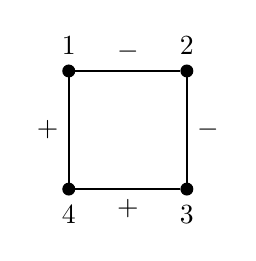
\begin{tikzpicture}[
				vertex/.style={draw, circle, inner sep=0pt, minimum size=.15cm, fill=black},
				edge/.style={thick}
				]
				% Nodes
				\node[vertex,label=above:1] (v1) at(-.75,.75) {};
				\node[vertex,label=above:2] (v2) at( .75,.75) {};
				\node[vertex,label=below:3] (v3) at( .75,-.75) {};
				\node[vertex,label=below:4] (v4) at(-.75,-.75) {};
				
				% Edges
				\draw[edge] (v1)--node[above] {$-$}(v2);
				\draw[edge] (v2)--node[right] {$-$}(v3);
				\draw[edge] (v3)--node[below] {$+$}(v4);
				\draw[edge] (v1)--node[left]  {$+$}(v4);
			\end{tikzpicture}
			\caption{Signed undirected graph $ G$ of $\mathcal{P}$.}
			\label{fign1}
		\end{minipage}
	\end{figure}
	
	Then $G$ is a cycle with exactly two negative edges and no maximal signed path of odd length. Therefore, $\mathcal{P}$ does not satisfy any of the three conditions
	of Theorem~\ref{xxth3}. Suppose that
	$$B=\begin{bmatrix}
		0&-a&0&b\\c&0&-d&0\\0&e&0&f\\g&0&h&0
	\end{bmatrix}\in \mathcal{Q}(\mathcal{P}),~\text{where}~a,b,c,d,e,f,g,h>0.$$
	Then the characteristic polynomial of $B$ is $\Ch_B(x)=x^4+(ac-bg+ed-fh)x^2-(acfh+adfg+ebch+ebdg)$. Take $f(x)=x^2+(ac-bg+ed-fh)x-(acfh+adfg+ebch+ebdg)$, then
	$$ 
	\sgn(f(x)) =  \begin{cases} 
		(+)-(*)(+)-(+) & \text{if} ~ x> 0 \\
		(+)-(*)(-)-(+) & \text{if} ~x<0,
	\end{cases} 
	$$ where $*$ denotes an arbitrary sign. Since $V_+(x)=1$ and $V_-(x)=1$, according to Descartes’ rule of signs, the number of positive and negative real roots of $f(x)$ is exactly one. Also, $\Ch_{B}(x)$ consists only of even powers of $x$, so by Lemma \ref{lem1}, $\In(B)=(1,1,2)$ for all $B\in \mathcal{Q}(\mathcal{P})$ and $\mathcal{P}$ requires a unique inertia.
\end{eg}

\begin{eg}\label{egxx0.6} Suppose that $\mathcal{P}\in \mathcal{Q}_4$ is an irreducible combinatorially symmetric sign pattern with a $0$-diagonal, whose underlying signed undirected graph is the graph $G$ given in Fig~\ref{xfig3.37}.
	\begin{figure}[H]
		\centering
		\begin{minipage}{.45\textwidth}
			\vspace{-1cm}
			\[
			\mathcal{P}=
			\begin{bmatrix}
				0 & + & 0 & + \\
				+ & 0 & + & 0 \\
				0 & + & 0 & + \\
				+ & 0 & + & 0
			\end{bmatrix}
			\]
		\end{minipage}
		\hspace{0.05\textwidth}
		\begin{minipage}{.45\textwidth}
			\centering
			\tikzset{node distance=1cm}
			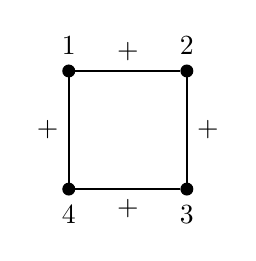
\begin{tikzpicture}[
				vertex/.style={draw, circle, inner sep=0pt, minimum size=.15cm, fill=black},
				edge/.style={thick}
				]
				% Nodes
				\node[vertex,label=above:1] (v1) at(-.75,.75) {};
				\node[vertex,label=above:2] (v2) at( .75,.75) {};
				\node[vertex,label=below:3] (v3) at( .75,-.75) {};
				\node[vertex,label=below:4] (v4) at(-.75,-.75) {};
				
				% Edges
				\draw[edge] (v1)--node[above] {$+$}(v2);
				\draw[edge] (v2)--node[right] {$+$}(v3);
				\draw[edge] (v3)--node[below] {$+$}(v4);
				\draw[edge] (v1)--node[left]  {$+$}(v4);
			\end{tikzpicture}
			\caption{Signed undirected graph $ G$ of $\mathcal{P}$.}
			\label{xfig3.37}
		\end{minipage}
	\end{figure}
	
	Then $G$ is a cycle with no negative edges and no maximal signed path of odd length. Therefore, $\mathcal{P}$ does not satisfy any of the three conditions
	of Theorem~\ref{xxth3}. However, consider	$$\begin{bmatrix}
		0&a&0&b\\ c&0&d&0\\ 0&e&0&f\\ g&0&h&0
	\end{bmatrix}\in \mathcal{Q}(\mathcal{P}), ~\text{where}~ a,b,c,d,e,f,g,h>0.$$ \begin{itemize}
		\item[i.] Let $B_1 \in \mathcal{Q}(\mathcal{P})$ with $a = b = c = d = e = f = g = h = 1$. Then $\sigma(B_1) = \{0, 0, 2, -2\}$, and $\In(B_1) = (1, 1, 2)$.
		\item[ii.] Let $B_2 \in \mathcal{Q}(\mathcal{P})$ with $a = c = f = h = 2$ and $b=d=e=g = 1$. Then $\sigma(B_2) = \{3, 1, -1, -3\}$, and $\In(B_2) = (2, 2, 0)$.
	\end{itemize}
	
	Therefore, $\mathcal{P}$ does not require a unique inertia.
\end{eg}
%%%%%%%%%%%%%%%
The following example shows that if in condition (iii) of the previous theorem, $\mathcal{P}$ is of odd order, then it may require a unique inertia even if it contains a maximal signed path of odd length.

\begin{eg}\label{xeg1} Suppose that $\mathcal{P}\in \mathcal{Q}_3$ is an irreducible combinatorially symmetric sign patterns with a $0$-diagonal, whose underlying signed undirected graph is $G$ given in Fig.\ref{xfign1.9}.
	\begin{figure}[H]
		\centering
		\begin{minipage}{.45\textwidth}
			\vspace{-1cm}
			\[
			\mathcal{P}=
			\begin{bmatrix}
				0 & - & + \\
				+ & 0 & - \\
				+ & + & 0
			\end{bmatrix}
			\]
		\end{minipage}
		\hspace{0.05\textwidth}
		\begin{minipage}{.45\textwidth}
			\centering
			\tikzset{node distance=1cm}
			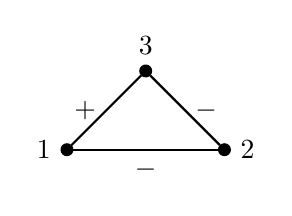
\begin{tikzpicture}[
				vertex/.style={draw, circle, inner sep=0pt, minimum size=.15cm, fill=black},
				edge/.style={thick}
				]
				% Nodes
				\node[vertex,label=left:1]  (v1) at(-1,0) {};
				\node[vertex,label=right:2] (v2) at( 1,0) {};
				\node[vertex,label=above:3] (v3) at( 0,1) {};
				
				% Edges
				\draw[edge] (v1)--node[below] {$-$}(v2);
				\draw[edge] (v2)--node[right] {$-$}(v3);
				\draw[edge] (v3)--node[left]  {$+$}(v1);
			\end{tikzpicture}
			\caption{Signed undirected graph $ G$ of $\mathcal{P}$.}
			\label{xfign1.9}
		\end{minipage}
	\end{figure}
	
	Then $G$ is a cycle containing a maximal signed path of odd length. However, $\mathcal{P}$ is a sign nonsingular sign pattern of odd order, by Theorem \ref{nth0.11}, $\mathcal{P}$ requires a unique inertia.
\end{eg}
%%%%%%%%%%%%%%%%%%%




The following are examples of sign patterns that satisfy conditions (i), (ii), and (iii) of Theorem~\ref{xxth3}, respectively, and therefore do not require a unique inertia.

\begin{eg}
	Let $\mathcal{P}\in \mathcal{Q}_4$ be an irreducible combinatorially symmetric sign pattern with a $0$-diagonal, whose underlying undirected graph is $G$ as in Example~\ref{xxeg1}. Since $G$ is a cycle with exactly one negative edge, so by Theorem~\ref{xxth3}(i), $\mathcal{P}$ does not require a unique inertia.
\end{eg}

\begin{eg} Suppose that $\mathcal{P}\in \mathcal{Q}_4$ is an irreducible combinatorially symmetric sign pattern with a $0$-diagonal, whose underlying signed undirected graph is the graph $G$ given in Fig~\ref{xfig3.3}.
	\begin{figure}[H]
		\centering
		\begin{minipage}{.45\textwidth}
			\vspace{-1cm}
			\[
			\mathcal{P}=
			\begin{bmatrix}
				0 & + & 0 & - \\
				- & 0 & + & 0 \\
				0 & - & 0 & + \\
				+ & 0 & - & 0
			\end{bmatrix}
			\]
		\end{minipage}
		\hspace{0.05\textwidth}
		\begin{minipage}{.45\textwidth}
			\centering
			\tikzset{node distance=1cm}
			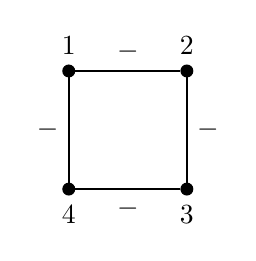
\begin{tikzpicture}[
				vertex/.style={draw, circle, inner sep=0pt, minimum size=.15cm, fill=black},
				edge/.style={thick}
				]
				% Nodes
				\node[vertex,label=above:1] (v1) at(-.75,.75) {};
				\node[vertex,label=above:2] (v2) at( .75,.75) {};
				\node[vertex,label=below:3] (v3) at( .75,-.75) {};
				\node[vertex,label=below:4] (v4) at(-.75,-.75) {};
				
				% Edges
				\draw[edge] (v1)--node[above] {$-$}(v2);
				\draw[edge] (v2)--node[right] {$-$}(v3);
				\draw[edge] (v3)--node[below] {$-$}(v4);
				\draw[edge] (v1)--node[left]  {$-$}(v4);
			\end{tikzpicture}
			\caption{Signed undirected graph $ G$ of $\mathcal{P}$.}
			\label{xfig3.3}
		\end{minipage}
	\end{figure}
	
	Then $G$ is a cycle with all edges negatively signed, so by Theorem~\ref{xxth3}(ii), $\mathcal{P}$ does not require a unique inertia.
\end{eg}

\begin{eg}\label{xxeg3.9} Suppose that $\mathcal{P}\in \mathcal{Q}_4$ is an irreducible combinatorially symmetric sign pattern with a $0$-diagonal, whose underlying signed undirected graph is $G$ given in Fig.\ref{xnfig2}.
	
	\begin{figure}[H]
		\centering
		\begin{minipage}{.45\textwidth}
			\vspace{-1cm}
			\[
			\mathcal{P}=
			\begin{bmatrix}
				0 & + & 0 & + \\
				- & 0 & + & 0 \\
				0 & + & 0 & + \\
				+ & 0 & - & 0
			\end{bmatrix}
			\]
		\end{minipage}
		\hspace{0.05\textwidth}
		\begin{minipage}{.45\textwidth}
			\centering
			\tikzset{node distance=1cm}
			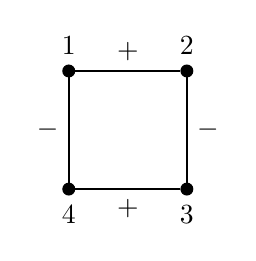
\begin{tikzpicture}[
				vertex/.style={draw, circle, inner sep=0pt, minimum size=.15cm, fill=black},
				edge/.style={thick}
				]
				% Nodes
				\node[vertex,label=above:1] (v1) at(-.75,.75) {};
				\node[vertex,label=above:2] (v2) at( .75,.75) {};
				\node[vertex,label=below:3] (v3) at( .75,-.75) {};
				\node[vertex,label=below:4] (v4) at(-.75,-.75) {};
				
				% Edges
				\draw[edge] (v1)--node[above] {$+$}(v2);
				\draw[edge] (v2)--node[right] {$-$}(v3);
				\draw[edge] (v3)--node[below] {$+$}(v4);
				\draw[edge] (v1)--node[left]  {$-$}(v4);
			\end{tikzpicture}
			\caption{Signed undirected graph $ G$ of $\mathcal{P}$.}
			\label{xnfig2}
		\end{minipage}
	\end{figure}
	Then $G$ is a cycle with a maximal signed path of odd length, so by Theorem~\ref{xxth3}(iii), $\mathcal{P}$ does not require a unique inertia.
\end{eg}





We use the following lemma to determine specific patterns or structures that an irreducible combinatorially symmetric sign pattern with a $0$-diagonal containing cycles cannot have if it requires a unique inertia.

%We use the following lemma to identify certain patterns or structures an irreducible combinatorially symmetric sign pattern with a $0$-diagonal and with cycles cannot have if it requires a unique inertia.


%  We use the following result to derive necessary conditions under which irreducible combinatorially symmetric sign patterns whose underlying signed undirected graph contains exactly one cycle require a unique inertia.

\begin{lemma}\label{l28}
	
	Let $\mathcal{P}\in \mathcal{Q}_n$ be an irreducible combinatorially symmetric sign pattern with a $0$-diagonal, whose underlying signed undirected graph is $G$ and the signed directed graph is $D$. Suppose that $G$ has exactly one cycle $\mathcal{C}=u_1u_2\cdots u_k$ of length $k$ and the distance of $\mathcal{C}$ from any leaf in $G$ is even. Then the maximum length of a composite cycle in $D$ is equal to the sum of the length of $\mathcal{C}$ and the maximum length of a composite cycle in $D\setminus V(\mathcal{C})$.       
\end{lemma}

\begin{proof} Let $D'=D\setminus V(\mathcal{C})$. If $G$ has no leaf, then there is nothing to prove. Suppose that $G$ has at least one leaf, then we prove this result by using induction on $m$, where $m$ is the number of leaves in $G$. For $m=1$, let $P=\{v_0,v_1\}\{v_1,v_2\}\cdots \{v_{2r-1},v_{2r}\}$ be the path from a vertex $v_0$ of $\mathcal{C}$ to the leaf $v_{2r}$ in $G$. Then $\bar{\Gamma}=\gamma\gamma_1\gamma_3\cdots\gamma_{2r-1},$ is a composite cycle with maximum length in $D$, 
	where $\gamma$ is the directed cycle $(u_1u_2\cdots u_k)$ and each $\gamma_i$ is a directed $2$-cycle $(v_i,v_{i+1})$ for $i=1,3,...,2r-1$. Consider
	$$\Gamma=\gamma_1\gamma_3\cdots\gamma_{2r-1},$$ 
	then $\Gamma$ is a composite cycle with maximum length in $D'$. So, the result is true for $m=1$.
	
	Suppose that the result holds
	for all $m$, $m \leq t-1$, $t \geq 2$.
	For $m = t$, let $u$ be a leaf in $G$ such that $\dist(u,\mathcal{C})$ is maximum. Let $v$ be the unique neighbour of $u$, then $v\notin V(\mathcal{C})$.
	
	\textbf{Case-1:} $v$ is adjacent to more than one leaf in $G$.\\
	Let $P_1=\{v_0,v_1\}\{v_1,v_2\}\cdots \{v_{2r},v\}\{v,u\}$ be a path from a vertex $v_0$ of $\mathcal{C}$ to $u$ such that none of $v_1,v_2,...,v_{2r}$ is in $V(\mathcal{C})$ and let $w$ be a neighbour of $v$ which is not in $P_1$. 
	\begin{figure}[H]
		\tikzset{node distance=1cm}
		\centering
		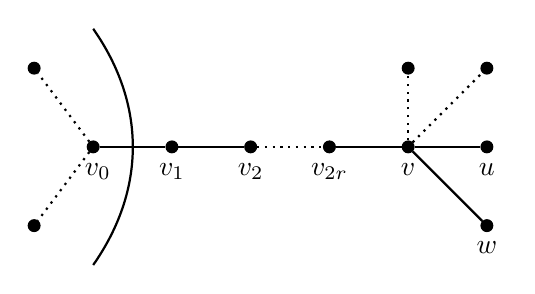
\begin{tikzpicture}
			\tikzstyle{vertex}=[draw, circle, inner sep=0pt, minimum size=.15cm, fill=black]
			\tikzstyle{edge}=[,thick]
			\node[vertex,label=below:$~v_0$](v1)at(0,0){};
			\node[vertex,label=below:$v_1$](v7)at(1,0){};
			\node[vertex,label=below:$v_2$](v8)at(2,0){};
			\node[vertex,label=below:$v_{2r}$](v9)at(3,0){};
			\node[vertex,label=below:$v$](v10)at(4,0){};
			\node[vertex,label=below:$u$](v11)at(5,0){};
			\node[vertex,label=below:$w$](v12)at(5,-1){};
			\node[vertex](v13)at(-0.75,1){};
			\node[vertex](v14)at(-0.75,-1){};
			\node[vertex] (v15) at (5,1) {};
			\node[vertex] (v16) at (4,1) {};
			\draw[thick]   (0,1.5) to [bend left=35] node[left] {$ $} (0,-1.5);
			\draw[edge](v1)--node[]{$ $}(v7);
			\draw[edge](v7)--node[]{$ $}(v8);
			\draw[thick, dotted](v8)--node[]{$ $}(v9);
			\draw[edge](v9)--node[]{$ $}(v10);
			\draw[edge](v10)--node[]{$ $}(v11);
			\draw[edge](v10)--node[]{$ $}(v12);
			\draw[thick, dotted](v1)--node[]{$ $}(v13);
			\draw[thick, dotted](v1)--node[]{$ $}(v14);
			\draw[thick, dotted](v10)--node[]{$ $}(v15);
			\draw[thick, dotted](v10)--node[]{$ $}(v16);
			
		\end{tikzpicture}
		\caption{$G$}	
	\end{figure}
	%  Let $G'=G\setminus\{u\}$, then $G'$ has $t-1$ leaves and the distance of each leaf in $G'$ to $\mathcal{C}$ is even. So, by the induction hypothesis there exists a composite cycle $\Gamma'$ of length $l$ with maximum length in $(D\setminus \{u\})\setminus V(\mathcal{C})$ such that the maximum length of a composite cycle in $D\setminus\{u\}$ is equal to $k+l$.
	%the sum of the length of $\mathcal{C}$ and the length of $\mathcal{M'}$. 
	
	Let $\Gamma_1, \Gamma_2$ be composite cycles of maximum length in $D, D'$, respectively. To show $l(\Gamma_1)=k+l(\Gamma_2)$. If $(v,u)\in \Gamma_1~\text{or}~\Gamma_2$, then replace $(v,u)$ by $(v,w)$ in $\Gamma_1,\Gamma_2$. Then $\Gamma_1,\Gamma_2$ are composite cycles in $D\setminus\{u\}$. Since $G\setminus\{u\}$ has $t-1$ leaves and the distance of each leaf to $\mathcal{C}$ in $G\setminus\{u\}$ is even, so by the induction hypothesis $l(\Gamma_1)=k+l(\Gamma_2)$.  If $(v,u)\notin \Gamma_1,\Gamma_2$, then $\Gamma_1$, $\Gamma_2$ are also composite cycles in $D \setminus \{u\}$, and hence the result follows.
	
	%  Since $v$ is adjacent to more than one leaf of $G$, if $\Gamma$ is a composite cycle with maximum length $r$ in $D'=D\setminus V(\mathcal{C})$, then \textbf{$\{\Gamma\setminus((u,v)\cup (v,v_{2r}))\}\cup\{(v,w)\}$}****$\{\Gamma\setminus\{(u,v),(v,v_{2r})\}\}\cup(v,w)$ is also a composite cycle with length $r$ in $D'$, $D'\setminus \{u\}$, therefore, $r=l$. Similarly, the maximum length of a composite cycle in $D$ is equal to the maximum length of a composite cycle in $D\setminus\{u\}$, which is equal to $k+l$.
	
	
	
	%$\mathcal{M'}$ is also a composite cycle with maximum length in $D\setminus V(\mathcal{C})$ and the maximum length of a composite cycle in $D$ is also equal to the sum of the length of $\mathcal{C}$ and the length of $\mathcal{M'}$.
	
	\textbf{Case-2:} $v$ is adjacent to exactly one leaf in $G$.\\
	Similarly, let $P_1=\{v_0,v_1\}\{v_1,v_2\}\cdots \{v_{2r},v\}\{v,u\}$ be a path from a vertex $v_0$ of $\mathcal{C}$ to $u$ such that none of $v_1,v_2,...,v_{2r}$ are in $V(\mathcal{C})$. 
	\begin{figure}[H]
		\tikzset{node distance=1cm}
		\centering
		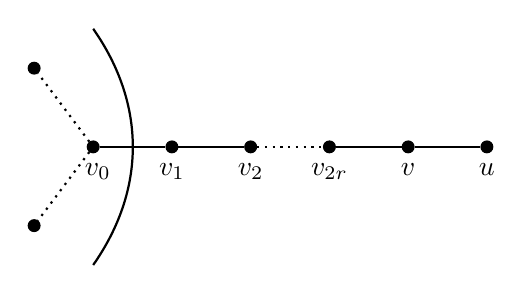
\begin{tikzpicture}
			\tikzstyle{vertex}=[draw, circle, inner sep=0pt, minimum size=.15cm, fill=black]
			\tikzstyle{edge}=[,thick]
			\node[vertex,label=below:$~v_0$](v1)at(0,0){};
			\node[vertex,label=below:$v_1$](v7)at(1,0){};
			\node[vertex,label=below:$v_2$](v8)at(2,0){};
			\node[vertex,label=below:$v_{2r}$](v9)at(3,0){};
			\node[vertex,label=below:$v$](v10)at(4,0){};
			\node[vertex,label=below:$u$](v11)at(5,0){};
			\node[vertex](v13)at(-0.75,1){};
			\node[vertex](v14)at(-0.75,-1){};
			
			\draw[thick] (0,1.5) to [bend left=35] node[left] {$ $} (0,-1.5);
			
			\draw[edge](v1)--node[]{$ $}(v7);
			\draw[edge](v7)--node[]{$ $}(v8);
			\draw[thick, dotted](v8)--node[]{$ $}(v9);
			\draw[edge](v9)--node[]{$ $}(v10);
			\draw[edge](v10)--node[]{$ $}(v11);	
			\draw[thick, dotted](v1)--node[]{$ $}(v13);
			\draw[thick, dotted](v1)--node[]{$ $}(v14);
		\end{tikzpicture}
		\caption{$G$}
	\end{figure}
	Let $\Gamma_1, \Gamma_2$ be composite cycles of maximum length in $D, D'$, respectively. Then either $(v,u) \in \Gamma_1$ (respectively, $\Gamma_2$), or $(v_{2r},v) \in \Gamma_1$ (respectively, $\Gamma_2$). If $(v_{2r},v)$ occurs in any one of $\Gamma_1, \Gamma_2$, replace it with $(v,u)$. Let $\Gamma_1'=\Gamma_1\setminus(v,u)$ and $\Gamma_2'=\Gamma_2\setminus(v,u)$. To prove the lemma, it is enough to show that $l(\Gamma_1')=k+l(\Gamma_2')$.  
	
	
	
	%If $\Gamma$ is also a composite cycle with maximum length $l$ in $D'$, then \textbf{$\Gamma'=(\Gamma\setminus((v_{2r},v)\cup(v,u)))\cup(v,u)$}******$\Gamma'=\{\Gamma\setminus\{(v_{2r},v),(v,u)\}\}\cup(v,u)$ is a composite cycle of length $l$ in $D'$ and the length of \textbf{$\Gamma\setminus((v_{2r},v)\cup(v,u))$}*****$\Gamma\setminus\{(v_{2r},v),(v,u)\}$ is $l-1$ which is the maximum length of a composite cycle in $D'\setminus\{u,v\}$.
	%So, there exists a composite cycle $\mathcal{M}'$ of $D'\setminus\{u,v\}$ of maximum length such that $\mathcal{M}'\cup (u,v)$ gives a composite cycle of maximum length in $D'$. 
	%Similarly, there exists a maximum length cycle $\mathcal{C}'$ in $D\setminus\{u,v\}$ such that $\mathcal{C}'\cup (u,v)$ gives a composite cycle of maximum length in $D$. Also, the distance of any leaf in $G\setminus\{u,v\}$ from $\mathcal{C}$ is even. To prove the result, it is enough to prove it for $G_1=G\setminus\{u,v\}$ and $D_1=D\setminus\{u,v\}$.
	
	
	%if $\mathcal{M}'$ is a composite cycle with maximum length in $D'\setminus \{u,v\}$, then $\mathcal{M}'\cup(v,u)$ forms a composite cycle with maximum length in $D'$. Similarly, if $\mathcal{C}_1$ is a composite cycle with a maximum length in $D\setminus\{u,v\}$, then $\mathcal{C}_1\cup(v,u)$ forms a composite cycle with a maximum length in $D$. So, it is enough to show the corresponding result for $D\setminus\{u,v\}$.
	
	If $v_{2r}$ is not a leaf of $G_1=G\setminus\{u,v\}$, then $G_1$ has $t-1$ leaves. Then, by the induction hypothesis, the result follows.
	%there is a composite cycle $\mathcal{M}_1$ with a maximum length in $(D\setminus\{u,v\})\setminus V(\mathcal{C})$ such that the maximum length of the composite cycle in $D\setminus\{u,v\}$ is equal to the sum of the length of $\mathcal{C}$ and the length of $\mathcal{M}_1$. 
	%Therefore, if $\mathcal{M}=\mathcal{M}_1\cup (u,v)$, then $\mathcal{M}$ forms a composite cycle with maximum length in $D\setminus V(\mathcal{C})$ and the maximum length of the composite cycle in $D$ is equal to the sum of the length of $\mathcal{C}$ and the length of $\mathcal{M}$.
	If $v_{2r}$ is a leaf of $G_1$, then apply the previous arguments with $D$ replaced by $D\setminus\{u,v\}$.
	
	
	
	
	%\\
	%\textbf{Subcase-1:} There is no such path from $v_{2r-1}$ to any leaf of $G\setminus\{u,v\}$ that does not share edges with $P_1$.\\
	
	
	%Then consider $\{D\setminus \{u,v\}\}\setminus\{v_{2r,}v_{2r-1}\}$ and repeat the above process.\\
	%\textbf{Subcase-2:} There is a path form $v_{2r-1}$ to a leaf of $G\setminus\{u,v\}$ that does not share edges** with $P_1$.\\ 
	
	
	%Let $u'$ be a leaf in $G\setminus\{u,v\}$ such that $\dist(u',v_{2r-1})$ is maximum and the shortest path from $u'$ to $v_{2r-1}$ in $G\setminus\{u,v\}$ does not share edges with $P_1$.
	%Then, apply the argument of the previous cases with $D$ replaced by $D\setminus\{u,v\}$
	%and $u$ replaced by $u'$.
	
	%Since $\dist(u',\mathcal{C})$ is even, $\dist(u',v_{2r-1})$ is odd. If $\dist(u',v_{2r-1})=1$, then similarly as in case-1, the result in hold. If $\dist(u',v_{2r-1})>1$, then we apply the previous argument on $u'$.\\
	
	After a finite number of steps, the above process of deleting edges gives a signed undirected graph $G_p$ with fewer than $t$ leaves. Let $D_p$ be the signed directed graph corresponding to $G_p$. By the induction hypothesis, there exists a composite cycle $\Gamma_p$ of maximum length in $D_p\setminus V(\mathcal{C})$ such that the maximum length of a composite cycle in $D_p$ is equal to the sum of the length of $\mathcal{C}$ and the length of $\Gamma_p$, so the result follows. %By adding the $2$-cycles corresponding to the deleted signed edges of $G$ with $\bar{\mathcal{M}}$, we obtained the required result.
\end{proof}

\begin{thebibliography}{99}
\bibitem[4]{1} 	C.A. Eschenbach, F.J. Hall, Z. Li. Eigenvalue frequency and consistent sign pattern matrices. \textit{Czechoslovak Math. J.}, 44 (119), 461–479, 1994.
	
	
	
	
	
	
	
	
	
\bibitem[5]{2001}   F.J.  Hall,  Z.  Li,  and  D.  Wang.   Symmetric sign pattern matrices that require unique inertia. \textit{Linear Algebra Appl.},338(1–3):153–169, 2001.
	
\bibitem[6]{2001a}  F.J. Hall and Z. Li.  Inertia sets of symmetric sign pattern matrices. \textit{J. Chin. Univ.}, 10(2):226–240, 2001.
	
	
\bibitem[7]{2018}  J.C.H. Lin, D.D. Olesky, and P. van den Driessche. Sign patterns requiring a unique inertia. \textit{Linear Algebra Appl.}, 546:67{85, 2018}.
	
\bibitem[8]{2024}  Rana, P. and Bandopadhyay, S., 2024. Some symmetric sign patterns requiring unique inertia. The Electronic Journal of Linear Algebra, 40, pp.396-417.
\end{thebibliography}
\end{document}
